\documentclass[conference,compsoc]{IEEEtran}

\raggedbottom

\ifCLASSOPTIONcompsoc
  % IEEE Computer Society needs nocompress option
  % requires cite.sty v4.0 or later (November 2003)
  \usepackage[nocompress]{cite}
\else
  % normal IEEE
  \usepackage{cite}
\fi


\usepackage[T1]{fontenc}
\usepackage{amsmath}
\usepackage{graphicx}
\usepackage{booktabs}
\usepackage{microtype}
\usepackage{pgfplots}
\usepackage{pgfplotstable}
\usepackage{caption}
\usepackage{multirow}
\usepackage{url}
\usepackage{float}
\usepgfplotslibrary{statistics}
\pgfplotsset{compat=1.18}

\def\BibTeX{{\rm B\kern-.05em{\sc i\kern-.025em b}\kern-.08em
    T\kern-.1667em\lower.7ex\hbox{E}\kern-.125emX}}

\makeatletter
\newcommand{\linebreakand}{%
  \end{@IEEEauthorhalign}
  \hfill\mbox{}\par
  \mbox{}\hfill\begin{@IEEEauthorhalign}
}
\makeatother

\hyphenation{op-tical net-works semi-conduc-tor}

\begin{document}
% \motto{This is my motto.}
\title{HiCWE: Bi-Encoder-based CWE Classification}
\author{
\IEEEauthorblockN{Anonymous Authors}
\IEEEauthorblockA{
    \textit{Anonymous Institution} \\
    Anonymous Email
}
}
\maketitle

% \author{

% \IEEEauthorblockN{Person A}
% \IEEEauthorblockA{
%     \textit{Some University} \\
%     email@email.com
% }

% \and
% \IEEEauthorblockN{Person B}
% \IEEEauthorblockA{
%     \textit{Some University} \\
%     email@email.com
% }

% \and
% \IEEEauthorblockN{Person C}
% \IEEEauthorblockA{
%     \textit{Some University} \\
%     email@email.com
% }

% \and
% \IEEEauthorblockN{Person D}
% \IEEEauthorblockA{
%     \textit{Some University} \\
%     email@email.com
% }
% }
% \maketitle


%%%%%%%%%%%%%%%%%%%%%%%
%%%%
\begin{abstract}
Automatically mapping Common Vulnerabilities and Exposures
(CVEs) to Common Weakness Enumeration (CWE) categories is
essential for understanding software vulnerabilities and
supporting vulnerability management. However, the official CWE
assignments may be missing or delayed, and automated
classification remains challenging due to overlapping
weakness definitions and the hierarchical structure of CWE.

We propose HiCWE, a hierarchy-aware
contrastive bi-encoder that automatically maps CVE
descriptions to CWE categories through semantic retrieval.
Unlike fixed-label classifiers and generative language
models, HiCWE learns representations of CVE descriptions
and CWE definitions in a shared embedding space,
incorporating hierarchical relationships during training to
structure the candidate space.

Evaluated on temporally separated CVE datasets, HiCWE
achieves 78.9\% top-1 accuracy for fine-grained CWE
classification and 82.0\% for category identification,
outperforming the evaluated baseline encoders and a
published classifier at the fine-grained level.
We further conduct an empirical study of 192,788 CVEs,
demonstrating the remaining coverage gap in CWE assignments
and the usefulness of historical CWE exploitation patterns
for vulnerability prioritization. Our results show that
hierarchy-aware semantic retrieval supports automated
CVE-to-CWE mapping and can aid vulnerability analysis and
prioritization.
\end{abstract}

%no keywords

% \begin{IEEEkeywords}
% Common Vulnerabilities and Exposures (CVE),
% Common Weakness Enumeration (CWE),
% Large Language Models,
% Vulnerability Prioritization,
% Exploitability Analysis
% \end{IEEEkeywords}
%%%%%%%%%%%%%%%%%%%%%%%%%%%%%%%%%%%%%%%%%%%%

\IEEEpeerreviewmaketitle

\section{Introduction}
\label{sec:introduction}

The Common Vulnerabilities and Exposures (CVE) system
provides standardized descriptions of publicly disclosed
vulnerabilities, while the Common Weakness Enumeration
(CWE) categorizes their underlying weaknesses.
Mapping CVEs to CWEs supports vulnerability analysis,
root-cause identification, and remediation. CWE information
may also contribute to vulnerability prioritization,
as severity scores do not necessarily reflect the
likelihood of exploitation in the wild
\cite{allodi2014comparing, jacobs2023epss}.
However, official CWE assignments may be missing or
delayed, motivating automated CVE-to-CWE mapping.

Existing approaches include keyword-based and
text-similarity methods \cite{albanese2024cve2cwe},
BERT-based classifiers \cite{das2021v2w},
and more recent transformer-based and generative
large language model (LLM) approaches \cite{mosievskiy2026roberta,liu2023not,simonetto2026knowing}.
Despite promising results, accurate mapping remains
challenging because CVE descriptions are often
incomplete, CWE definitions overlap semantically,
and weaknesses are organized hierarchically.
Furthermore, conventional classifiers typically
rely on fixed output labels, while generative
LLMs may produce incorrect CWE identifiers or
confuse related weakness categories.

To address these challenges, we propose
\textbf{HiCWE}, a hierarchy-aware contrastive
bi-encoder for automated CVE-to-CWE mapping.
HiCWE formulates classification as a semantic
retrieval task, learning representations of CVE
descriptions and CWE definitions in a shared
embedding space. By incorporating hierarchical
relationships during contrastive training,
HiCWE improves discrimination between related
weaknesses. Unlike fixed-label classifiers,
it directly ranks CWE definitions, allowing
the candidate set to be updated without
retraining a classification head.

We evaluate HiCWE using temporally separated
CVE datasets, training on 1999--2021 data
and testing on 2023--2025 vulnerabilities.
We compare its performance with baseline
encoders, an existing CWE classifier~\cite{mullikencwepredictor}, and
generative LLM-based approaches. We also
conduct an empirical study of 192,788 CVEs
to investigate CWE assignment availability,
mapping stability, and historical exploitation
patterns, establishing the practical motivation
for timely and accurate CWE classification.

The main contributions of this paper are:

\begin{itemize}
    \item \textbf{Automated CVE-to-CWE mapping:}
    We introduce HiCWE, a hierarchy-aware
    contrastive bi-encoder that incorporates
    CWE relationships into semantic retrieval
    for fine-grained weakness classification.

    \item \textbf{Experimental evaluation:}
    We evaluate HiCWE on temporally separated
    datasets, achieving 78.9\% top-1 fine-grained
    CWE accuracy and 82.0\% category-level
    accuracy. We also investigate generative
    LLM-based mapping under different prompting
    configurations.

    \item \textbf{Empirical motivation:}
    We analyze CWE assignment delays, missing
    mappings, and historical exploitation patterns,
    demonstrating the value of timely CWE
    information and its potential usefulness
    for vulnerability prioritization.
\end{itemize}

To preserve author anonymity, the fine-tuned models will be released on Hugging Face after the review process. The source code\footnote{\url{https://anonymous.4open.science/r/CWE_CVE_Mapping-D776/README.md}} and demo\footnote{\url{https://demo_tbd_url.com}} are available in our anonymized repository.


\section{Background}
\label{sec:background}

\subsection{Early Vulnerability Prioritization}

The increasing number of publicly disclosed software
vulnerabilities presents a significant challenge for
security teams, which must prioritize remediation
efforts with limited resources. Vulnerability
prioritization has traditionally relied on the
Common Vulnerability Scoring System (CVSS).
However, vulnerability severity does not necessarily
reflect the likelihood of exploitation in the wild.
Consequently, researchers have investigated
alternative approaches that incorporate
exploitation-related information into vulnerability
prioritization.

The Exploit Prediction Scoring System (EPSS),
developed by Jacobs et al.~\cite{jacobs2021epss},
estimates the probability that an individual CVE
will be exploited. Sherif et al.~\cite{sherif2026kri}
combined threat, impact, and exposure information
into a Key Risk Indicator framework.
Our prior
work~\cite{khanmohammadi2025exploitabilitybirthmark}
introduced \textit{ExploitabilityBirthMark},
which predicts vulnerability exploitability using
information available at disclosure.
Jiang et al.~\cite{jiang2025survey} surveyed
the broader development of dynamic vulnerability
prioritization approaches incorporating
exploitation-related information.

Although these approaches contribute to more
informed vulnerability prioritization, they
primarily focus on individual CVEs. An alternative
source of information is the historical exploitation
behavior of the underlying software weaknesses.
Unlike vulnerability-specific indicators, which
may be unavailable or incomplete at disclosure,
historical weakness-level information can be
estimated from previously disclosed vulnerabilities.

This observation motivates our first research
objective: determining whether historical CWE
exploitation patterns are sufficiently stable
and informative to support the early prioritization
of newly disclosed vulnerabilities.

\subsection{Historical Exploitability at the CWE Level}

CWE provides
a taxonomy of software and hardware weaknesses
that can lead to vulnerabilities. While CVEs
identify individual vulnerabilities, CWE categories
describe recurring weaknesses that may affect
multiple products and systems. Consequently,
vulnerabilities associated with the same CWE
may exhibit common exploitation characteristics.

Previous research has investigated the measurement
and ranking of software weaknesses. Mell and
Gueye~\cite{mell2020suite} proposed metrics for
evaluating CWE categories based on vulnerability
frequency, severity, impact, and exploitability.
Galhardo et al.~\cite{galhardo2020measurements}
investigated the limitations of the MITRE CWE Top 25
ranking methodology~\cite{cwe_top25} and proposed
refinements to better balance exploitability
and impact.
A separate line of work has studied exploit prediction
at the level of individual vulnerabilities, where
weakness-related information appears as one input among
many. Bozorgi et al.~\cite{bozorgi2010beyond} trained
classifiers on vulnerability metadata and textual
features to predict exploitation, and Suciu et
al.~\cite{suciu2022expected} predicted the development
of functional exploits from a broad feature set.
EPSS~\cite{jacobs2021epss} likewise includes CWE among
its inputs, while Allodi and
Massacci~\cite{allodi2014comparing} showed through
case-control studies that CVSS severity is a weak
indicator of exploitation in the wild.
In these approaches, however, the CWE is one feature of
a vulnerability-level model and its marginal value is
not isolated. In contrast, we study CWE-level
exploitation history as a standalone, interpretable
signal, and  measure its temporal stability.


These studies highlight the value of
characterizing software weaknesses beyond
individual vulnerabilities. However, their
primary objective is to identify and rank
important weakness categories rather than
estimate the exploitation risk of newly
disclosed CVEs.

For historical CWE exploitability to serve as
a useful prioritization signal, two conditions
must be investigated. First, exploitation rates
must differ meaningfully across weakness
categories. Second, these differences must
exhibit sufficient temporal stability to provide
information about vulnerabilities disclosed
in subsequent years.

Therefore, our study examines the distribution
of real-world exploitation across CWE categories
and evaluates whether historical CWE exploitation
patterns retain predictive value over time.

\subsection{Automated CVE-to-CWE Mapping}
\label{subsec:automated_mapping}

A practical challenge in CWE-based vulnerability
prioritization is the availability of CWE
assignments. Newly disclosed CVEs may initially
lack specific CWE identifiers, preventing the
immediate use of historical weakness-level
exploitability information. Automated CVE-to-CWE
mapping addresses this limitation by identifying
the underlying weakness from the vulnerability
description.

Existing approaches include keyword-based
methods, supervised language models, generative
LLMs, and semantic
embedding-based retrieval.

\subsubsection{Keyword-Based Methods}

Keyword-based approaches identify weakness categories using predefined terms and patterns, such as SQL injection, cross-site scripting (XSS), and cross-site request forgery (CSRF). Although effective when vulnerability descriptions contain recognizable terminology, these methods are sensitive to wording, may produce false positives, and struggle with descriptions that lack distinctive keywords.

\subsubsection{Supervised Classification Methods}

Supervised approaches instead learn a mapping from descriptions to weakness labels and, unlike keyword rules, generalize beyond a fixed lexicon.

Das et al.~\cite{das2021v2w} proposed V2W-BERT, a hierarchical BERT-based framework that reports up to 97\% prediction accuracy for randomly partitioned data and up to 94\% for temporally partitioned data. The 97\% figure uses relaxed hierarchical matching; under strict exact matching the same model reaches 89.2\%.

Albanese et al.~\cite{albanese2024cve2cwe} proposed CVE2CWE, which represents each CWE using TF-IDF features extracted from historical CVE descriptions and applies cosine similarity to classify new vulnerabilities. It reaches 69.9\% top-1 over the 25 most frequent CWEs and 57.2\% over 50 CWEs, in both cases within a closed set containing only those labels.

More recently, Mosievskiy~\cite{mosievskiy2026roberta} fine-tuned a 125M-parameter RoBERTa-base classifier and reports 87.4\% top-1 over 205 CWE classes. That result is measured on an agreement-filtered test set that removes cases where NVD and AI-generated labels disagree; on the external CTI-Bench benchmark the same model reaches 75.6\% strict and 86.5\% hierarchy-aware top-1.

Because each study fixes its own label set, train/test split, and matching rule, these accuracies are not directly comparable to one another or to ours; we return to this point when interpreting our results in Section~\ref{sec:hicwe}.

A limitation shared by all of these supervised systems is that they operate over a predefined label set, so weaknesses absent from training cannot be predicted reliably. This matters because the CWE taxonomy evolves: HiCWE avoids retraining by adding new CWE descriptions to the index, whereas a fixed classification head must be retrained or extended.


\subsubsection{Generative LLM-Based Methods}

Generative LLMs offer a more flexible approach
by predicting CWE identifiers directly from
vulnerability descriptions through prompting.
Liu et al.~\cite{liu2023not} investigated
ChatGPT-based vulnerability mapping using
13,513 CVEs, reporting exact-match accuracies
of 50.88\% and 53.13\% under two prompting
strategies. When hierarchical relationships
were considered, parent-level agreement
increased to 72.20\% and 76.13\%,
respectively.

These results highlight the difficulty of
identifying precise CWE identifiers, even
when broader weakness categories are
correctly recognized.

Simonetto et al.~\cite{simonetto2026knowing}
further investigated CWE classification using
fine-tuned language models and hierarchical
information, reporting an approximately
five-percentage-point improvement in F1-score
over a supervised baseline.

Their comparison reported approximately
61\% weighted F1-score for a previously
evaluated prompted ChatGPT approach,
72\% for a supervised BiGRU-TextCNN baseline,
and 62\% for zero-shot GPT-3.5.
Their strongest LLM-based approach required
fine-tuning a 7-billion-parameter model,
with reported training costs of approximately
95 hours and 19.7 kWh, compared with
0.9 kWh for BERT.

Despite their flexibility, generative
approaches introduce several challenges.
Large models can require substantial
computational resources, while fine-tuned
classification approaches may still be
restricted to a limited set of CWE categories.
For example, Simonetto et
al.~\cite{simonetto2026knowing} focused on
the 57 most frequent CWE categories,
covering approximately 95\% of their
labeled CVEs, potentially limiting coverage
of rare and newly introduced weaknesses. Another challenge concerns potential data
contamination, as publicly available CVE
descriptions and CWE assignments may have
appeared in model pretraining corpora.
To mitigate this concern, Simonetto et al.~\cite{simonetto2026knowing}
constructed a separate evaluation dataset
of 2,777 CVEs published after the release
of their base model.

These limitations motivate the investigation
of computationally efficient approaches
that can identify precise weaknesses,
generalize to future vulnerabilities,
and accommodate changes to the CWE taxonomy.

\subsubsection{Semantic Embedding-Based Retrieval}

Embedding-based methods formulate CVE-to-CWE mapping as a semantic retrieval problem.
Rather than predicting CWE identifiers
through a fixed classification layer or
generating them as text, these approaches
represent CVE descriptions and CWE definitions
in a shared embedding space and rank candidate
weaknesses according to semantic similarity.

Haddad et al.~\cite{haddad2023automated}
investigated this direction by evaluating
Sentence-BERT and rankT5 models on a
manually annotated dataset of 4,012 CVEs.
Their results demonstrated improvements
over traditional information retrieval
and transformer-based baselines.

A key advantage of bi-encoder retrieval
architectures is that candidate CWE
definitions can be evaluated without
requiring a dedicated output neuron for
each weakness. This enables changes to
the candidate set without modifying
a fixed classification layer.
Furthermore, similarity scores can be
used to rank alternative CWE assignments,
although they should not be interpreted
as calibrated classification probabilities.

Nevertheless, semantic retrieval remains
challenging because CWE definitions can
overlap substantially, and vulnerabilities
may correspond to closely related weaknesses.
The hierarchical relationships among
CWE categories provide additional structural
information that may help distinguish
these semantically similar candidates.

This motivates the hierarchy-aware approach
we introduce next.


\section{Empirical Study}
\label{sec:dataset_methodology}

The objective of this empirical study is to investigate
the availability, consistency, and practical value of
CWE assignments in vulnerability analysis. In particular,
we examine two questions that motivate our research:
(1) whether the availability and quality of official
CVE-to-CWE mappings justify the development of automated
mapping approaches, and (2) whether historical CWE
exploitation patterns provide useful information for
predicting and prioritizing vulnerabilities exploited
in the wild.


\subsection{Data Sources}
To investigate these questions, we constructed a
dataset by integrating vulnerability metadata and
real-world exploitation evidence from multiple
publicly available and proprietary sources.
Figure~\ref{fig:empirical_study} illustrates
the datasets and their integration in our
empirical study.

The National Vulnerability Database (NVD) served
as the primary source of vulnerability information.
We collected CVE identifiers, vulnerability
descriptions, publication dates, CWE assignments,
and CVSS scores. We additionally used the NVD
API to gather the CVEs' change history to examine modifications
to CWE assignments, including their initial
availability and subsequent revisions.

To identify vulnerabilities exploited in the wild,
we integrated three complementary exploitation
datasets: the CISA Known Exploited Vulnerabilities
(KEV) catalog\footnote{
https://www.cisa.gov/known-exploited-vulnerabilities-catalog},
VulnCheck's exploitation dataset\footnote{
https://research.vulncheck.com/},
and GreyNoise's dataset of actively exploited
CVEs\footnote{https://www.greynoise.io}.
A CVE was labeled as exploited if it appeared
in at least one of these three sources.

After merging the datasets and removing duplicate
CVE--CWE pairs, the resulting dataset contained
192,788 unique CVEs, 768 distinct CWE categories,
and 3,097 CVEs identified as exploited in the wild.
These records provide the basis for examining
CWE assignment practices and constructing
historical exploitation profiles for individual
weakness categories.

\textbf{Empirical Study Design--}
We organized the empirical study into six
complementary analyses addressing the
availability, reliability, and exploitability
information associated with CWE mappings.

The first three findings examine the
characteristics of official CWE assignments.
Finding 1 investigates the delay between
CVE publication and the availability of
the initial CWE assignment, providing
evidence about the timeliness of weakness-level
information. Finding 2 examines how frequently
CWE mappings are revised and the time
elapsed before these revisions occur.
Finding 3 analyzes the number of CWE
assignments associated with each CVE,
including vulnerabilities with missing
or multiple weakness classifications.
Together, these analyses characterize
the practical challenges that automated
CVE-to-CWE mapping could help address.

The remaining three findings investigate
the relationship between CWE categories
and exploitation in the wild. Finding 4
examines the temporal stability of
historical CWE exploitation rates to
determine whether weakness-level
exploitation patterns persist across
consecutive years. Finding 5 identifies
CWE categories disproportionately
associated with observed exploitation
and evaluates the consistency of these
associations over time. Finding 6
assesses whether historical CWE
exploitation probabilities can be used
to rank vulnerabilities according to
their observed exploitation outcomes,
comparing CWE-based ranking performance
against random ranking.

These analyses provide complementary
evidence for assessing whether CWE
assignments contain useful information
for vulnerability exploitability
prediction and prioritization, and
whether improving their availability
through automated mapping could
offer practical benefits.

\textbf{Temporal Scope and Data Preparation--}
Different temporal subsets of the
dataset were used according to the
objectives of each analysis. Findings
1 and 2 focus on CVEs published in
2025 to reduce the influence of the
NVD processing backlog during 2024,
which affected the timeliness of
vulnerability analysis and metadata
updates. Finding 3 examines CVEs
published between 2020 and 2025
to characterize the distribution
of CWE assignments.

Finding 4 analyzes temporal CWE
exploitation patterns using CVEs
published between 2020 and 2026.
Finding 5 uses the complete merged
dataset to identify weakness
categories associated with elevated
exploitation in the wild. Finally,
Finding 6 employs a rolling temporal
evaluation covering 2021--2025,
using CVEs published in preceding
years to construct historical CWE
exploitation scores for ranking
CVEs published in each evaluation year.

Before analysis, duplicate CVE--CWE
pairs were removed. Generic or
non-informative CWE labels, including
\texttt{NVD-CWE-noinfo} and
\texttt{NVD-CWE-Other}, were excluded
where appropriate. Because individual
CVEs may be associated with multiple
CWEs, weakness-level exploitation
analyses were performed at the
CVE--CWE pair level, whereas analyses
of publication dates, assignment
delays, and mapping revisions were
performed at the CVE level.

\textbf{Statistical Analysis--}
Descriptive statistics, including
counts, percentages, means, medians,
quartiles, and standard deviations,
were used to characterize CWE
assignment patterns and exploitation
distributions.

To investigate associations between
CWE categories and exploitation,
we employed Fisher's exact test,
with Benjamini--Hochberg adjustment
to control the false discovery rate.
Temporal stability was evaluated
using Spearman's rank correlation
and linear regression, with bootstrap
confidence intervals where applicable.

For the vulnerability prioritization
experiment, ranking performance
was evaluated using PR-AUC,
ROC-AUC, Precision@$k$,
Recall@$k$, and NDCG@$k$.
Random ranking was used as a
baseline to assess whether historical
CWE exploitation information provides
additional discriminatory value.

This study establishes
the motivation for our subsequent
investigation of LLM-based CVE-to-CWE
mapping. The analyses first examine
whether official CWE assignments
are sufficiently timely and complete
for vulnerability management, and
then assess whether CWE information
contains meaningful historical
exploitation signals. Together,
these findings provide an empirical
basis for investigating automated
CWE classification as a means of
improving access to weakness-level
information and supporting its
potential use in exploitability
prediction and vulnerability
prioritization.
\begin{figure}[!t]
    \centering
    
    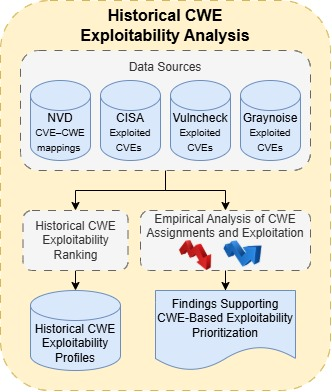
\includegraphics[width=0.8\columnwidth]{Figures/empirical_study.jpg}
    \caption{Data sources and their integration in the empirical study.}
    \label{fig:empirical_study}
\end{figure}

% \section{Historical CWE Exploitability Study}
% \subsection{Dataset and Methodology}
% \label{sec:dataset_methodology}



%  This empirical study combines vulnerability information from multiple publicly available sources to investigate the evolution of CWE mappings and historical exploitability patterns. Figure~\ref{fig:empirical_study} presents an overview of
% the empirical study, illustrating the datasets used.  The primary source of vulnerability metadata is the National Vulnerability Database (NVD), from which we collected CVE records, publication dates, CWE mappings, CVSS scores, and CVE change-history information. To study the evolution of CWE assignments after disclosure, we additionally used the NVD CVE Change History API, which records modifications made to CVE metadata, including the addition and revision of CWE mappings.

% To identify vulnerabilities exploited in the wild, we integrated three complementary exploitation datasets: the CISA Known Exploited Vulnerabilities (KEV) catalog\footnote{https://www.cisa.gov/known-exploited-vulnerabilities-catalog}, VulnCheck's exploitation dataset\footnote{https://research.vulncheck.com/}, and  a proprietary dataset of actively exploited CVEs created by the firm GreyNoise\footnote{ https://www.greynoise.io}. A CVE was considered exploited if it appears in at least one of these sources. After merging the datasets and removing duplicate CVE--CWE pairs, the final dataset contained 192,788 unique CVEs, 768 distinct CWE categories, and 3,097 CVEs known to have been exploited in the wild. These exploited CVEs were used to construct historical exploitability profiles for individual CWE categories.

% our study require different temporal subsets of the data. We analyze CVEs published in 2025, in Findings 1 and 2, to minimize the impact of the well-documented NVD processing backlog during 2024, which delayed vulnerability analysis and metadata publication. We examined the complete set of available CVE--CWE mappings in Finding 3, to characterize the distribution of weakness assignments. Finding 4 is based on analysis over temporal exploitability trends using CVEs published between 2020 and 2026, while for Finding 5, we used the complete merged dataset to identify weakness categories that are disproportionately associated with real-world exploitation. 

% Prior to analysis, duplicate CVE--CWE pairs were removed, and generic or non-informative CWE labels (\texttt{NVD-CWE-noinfo} and \texttt{NVD-CWE-Other}) were excluded where appropriate. Because a single CVE may be associated with multiple CWE identifiers, analyses involving weakness-level exploitability were performed at the CVE--CWE pair level, whereas analyses involving publication dates, CWE assignment delays, and CVSS scores were performed at the CVE level.


% \textbf{CWE Association with Exploitation:} To identify software weakness categories that are disproportionately associated with real-world exploitation, we combined CVE--CWE mappings from the National Vulnerability Database (NVD) with exploitation evidence from CISA Known Exploited Vulnerabilities (KEV), VulnCheck, and GreyNoise. For each CWE, we computed its exploitation rate, contribution to exploited CVEs, and odds ratio measuring the strength of association with exploitation. 
% Statistical significance was assessed using a one-sided Fisher's exact test, and $p$-values were adjusted using the Benjamini--Hochberg procedure to control the false discovery rate.
% To ensure robust estimates, only CWEs with at least 100 associated CVEs, at least 10 exploited CVEs, observations spanning at least three years, an odds ratio greater than one, and an adjusted $p$-value below 0.05 were retained. We further evaluated the temporal consistency of exploitation using the proportion of years in which a CWE was exploited and a stability score derived from the coefficient of variation of annual exploitation rates. Eligible CWEs were then ranked using a composite score combining exploitation rate (30\%), odds ratio (25\%), exploited-CVE count (25\%), temporal stability (10\%), and the percentage of years with observed exploitation (10\%). Finally, we compared the resulting ranking with the MITRE 2025 CWE Top 25 using set overlap, Jaccard similarity, and Spearman rank correlation, and performed sensitivity analyses under alternative minimum sample-size thresholds to evaluate the robustness of the findings.

% Throughout the empirical study, descriptive statistics are reported using counts, percentages, means, medians, quartiles, and standard deviations where appropriate. Depending on the research question, statistical analyses include Fisher's exact test to evaluate associations between CWE categories and exploitation, Spearman's rank correlation and linear regression to assess temporal stability, Friedman and Wilcoxon signed-rank tests to compare CVSS versions, and bootstrap confidence intervals where applicable. For analyses involving multiple hypothesis tests, $p$-values were adjusted using the Benjamini--Hochberg procedure to control the false discovery rate.

\subsection{Finding 1: Initial CWE Assignments Have Become Faster, but Substantial Delays Persist for Some CVEs}

To motivate the need for automated early CWE assignment, we first examine the delay between the public disclosure of a CVE and the availability of its corresponding CWE mapping. Indeed,  vulnerability prioritization often begins immediately after disclosure. However, CVEs are often published without an assigned CWE, a delay that hinders practitioners from leveraging weakness-level information during the critical early stages of vulnerability assessment. Quantifying these delays provides insight into the potential benefit of automatically predicting the underlying CWE using an LLM at disclosure time.

Figure~\ref{fig:cwe_assignment_delay} shows the distribution of delays for all CVEs, CVEs published between 2015--2025, and CVEs published in 2025. The distributions are highly right-skewed, with most vulnerabilities receiving a CWE assignment within a few days of publication. Across all CVEs, the median delay was 2.24 days, increasing slightly to 3.17 days for CVEs published between 2015 and 2025. In contrast, the median delay for 2025 CVEs was 0 days, indicating that at least half of newly disclosed vulnerabilities received a CWE assignment on the day of publication. Likewise, the upper quartile decreased from approximately eight days in the historical datasets to essentially zero days in 2025, demonstrating substantial improvements in the timeliness of CWE assignment.

Despite these improvements, a small number of vulnerabilities experience exceptionally long assignment delays, producing mean delays of 65.78, 24.05, and 12.81 days for the three datasets, respectively. These long-tail cases substantially inflate the averages and indicate that weakness-level information may remain unavailable for extended periods for some vulnerabilities. Because CWE is one of the features used by exploitability prediction systems such as EPSS, delays in obtaining an official CWE assignment postpone the availability of weakness-level information. Our automated approach addresses this limitation by inferring the underlying CWE immediately after CVE disclosure, enabling earlier vulnerability prioritization using historical weakness-level exploitability information.
\begin{figure}[!t]
    \centering
    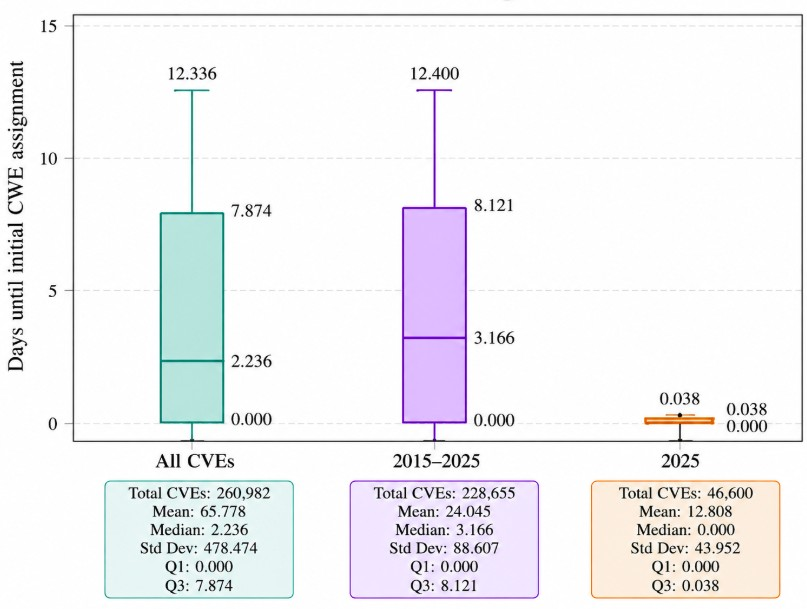
\includegraphics[width=\columnwidth]{Figures/figure 5.jpg}
    \caption{Distribution of delays between CVE publication
    and initial CWE assignment across three time periods.}
    \label{fig:cwe_assignment_delay}
\end{figure}


\subsection{Finding 2: CWE Assignments Are Rarely Revised, and Most Revisions Occur Shortly After Initial Assignment}

Among the 46,600 CVEs published in 2025, only 905 CVEs (around 2\%) experienced at least one change to their CWE mapping after the initial assignment. These updates accounted for 1,006 CWE change events, indicating that a small number of CVEs underwent multiple mapping revisions. Overall, the time lag between the initial CWE mapping and subsequent updates was very short, with a mean of 0.91 days and a median of 0 days, suggesting that most modifications occurred on the same day as the initial mapping. The distribution of update delays was highly concentrated in the first week: 987 (98.1\%) of all CWE change events occurred within 0–7 days, while only 7 (0.7\%) occurred between 8–30 days and 12 (1.2\%) occurred between 31–90 days. No CWE mapping changes were observed after 90 days. 

We limited our analysis to CVEs published in 2025 to avoid bias introduced by the well-documented NVD processing disruption in 2024~\cite{NVD2024Backlog,NIST2026NVD}. The NVD developed a substantial backlog of vulnerability evaluations starting in February 2024, which caused delays in the assignment and updating of metadata, including CWE mappings. If included in our analysis, these operational delays would have artificially inflated the observed time lag between the initial and subsequent CWE mappings.


\subsection{Finding 3: Most CVEs Are Associated with
a Single CWE, but Missing and Multiple Mappings Persist}

Table~\ref{tab:cwe_mapping_distribution_2020_2025} summarizes the number of CWE mappings assigned to each CVE published between 2020 and 2025. Among the 180,599 CVEs analyzed, the majority (138,343; 76.60\%) were associated with only one CWE. An additional 18,763 CVEs (10.39\%) were mapped to two CWEs, while only 918 CVEs (0.51\%) were associated with three or more CWEs.

A notable proportion of vulnerabilities (22,575; 12.50\%) had no specific CWE mapping, reflecting cases where the underlying weakness had not been identified or was recorded using non-informative classifications such as \texttt{NVD-CWE-noinfo} or \texttt{NVD-CWE-Other}. CVEs associated with four or more CWEs were extremely rare, accounting for fewer than 0.05\% of all vulnerabilities. The maximum number of CWE mappings observed for a single CVE was eight, occurring in only one case.

Overall, these results indicate that while most vulnerabilities can be characterized by a single software weakness, a non-negligible fraction involve multiple underlying weaknesses, suggesting that complex vulnerabilities may span multiple stages of a software flaw or affect several related weakness categories.


% \begin{table}[h]
% \centering
% \caption{Distribution of CVEs by Number of CWEs}
% \begin{tabular}{lrrr}
% \toprule
% \textbf{Number of Assigned CWEs} & \textbf{Number of CVEs} \\
% \midrule
% 1   & 282{,}798    \\
% 2   & 36{,}404       \\
% 3   & 1630        \\
% 4   & 134      \\
% 5   & 20        \\
% 6   & 7        \\
% 7   & 6       \\
% 8   & 1        \\
% \bottomrule
% \end{tabular}
% \end{table}


\begin{table}[t]
\centering
\scriptsize
\setlength{\tabcolsep}{3pt}
\caption{Distribution of the Number of CWE Mappings per CVE from 2020--2025}
\label{tab:cwe_mapping_distribution_2020_2025}
\begin{tabular}{lrr}
\toprule
\textbf{Number of Mapped CWEs} & \textbf{Number of CVEs} & \textbf{Percentage (\%)} \\
\midrule
0 & 22,575  & 12.50 \\
1 & 138,343 & 76.60 \\
2 & 18,763  & 10.39 \\
3 & 844      & 0.47 \\
4 & 57       & 0.03 \\
5 & 10       & 0.01 \\
6 & 3        & 0.00 \\
7 & 3        & 0.00 \\
8 & 1        & 0.00 \\
\midrule
\textbf{Total} & \textbf{180,599} & \textbf{100.00} \\
\bottomrule
\end{tabular}
\end{table}


% \begin{table}[H]
% \centering
% \caption{Distribution of the Number of CWE Mappings per CVEs in 2025}
% \label{tab:cwe_distribution}
% \begin{tabular}{lrr}
% \toprule
% \textbf{Number of CWE Mappings} & \textbf{Number of CVEs} & \textbf{Percentage (\%)} \\
% \midrule
% 0 & 3,528  & 7.85  \\
% 1 & 34,073 & 75.85 \\
% 2 & 6,904  & 15.37 \\
% 3 & 392    & 0.87  \\
% 4 & 18     & 0.04  \\
% 5 & 2      & 0.00  \\
% 6 & 2      & 0.00  \\
% 7 & 1      & 0.00  \\
% 8 & 1      & 0.00  \\
% \bottomrule
% \end{tabular}
% \end{table}




\subsection{Finding 4: Historical CWE Exploitability Exhibits Moderate Temporal Stability}

To evaluate the temporal stability of CWE exploitability profiles, we analyzed CVEs published between 2020 and 2026 and linked them with known exploitation-in-the-wild records from CISA KEV, VulnCheck, and Greynoise's exploitation dataset. To reduce instability caused by sparse observations, we restricted the analysis to CWE-year combinations containing at least 20 CVEs. This resulted in 908 CWE-year observations spanning 210 unique CWEs.

We used Spearman rank correlation to compare CWE exploitability rates between consecutive years. All six year-to-year comparisons exhibited statistically significant positive correlations ($p<0.001$), with correlation coefficients ranging from 0.388 (2022--2023) to 0.568 (2021--2022). Across all consecutive years, the mean Spearman correlation was 0.480, indicating moderate temporal stability in CWE exploitability profiles.

To determine whether historical exploitability predicts future exploitability, we compared exploitability rates in year $t$ with those in year $t+1$. The overall lagged Spearman correlation was 0.468 ($p<0.001$), with a bootstrap 95\% confidence interval of [0.396, 0.538], indicating a consistent positive relationship between historical and future exploitability. Linear regression further confirmed this relationship, producing a statistically significant positive slope of 0.364 ($p<0.001$) and an $R^2$ value of 0.184. Although historical exploitability explains only part of the variation in future exploitability, the results demonstrate that CWEs exhibiting higher exploitation rates in one year tend to remain relatively more exploitable in subsequent years.

Finally, we repeated the analysis using only the 76 CWEs that appeared in every year of the study period. The resulting Spearman correlations ranged from 0.450 to 0.641, consistently exceeding those obtained from the complete dataset. This finding suggests that exploitability profiles are even more stable for well-established CWEs that are consistently represented across years.

These results indicate that CWE exploitability profiles exhibit moderate but statistically significant temporal stability. Historical exploitation patterns, therefore, provide useful predictive information for estimating the future exploitability of vulnerability classes, although additional factors beyond CWE also influence whether individual vulnerabilities are exploited in the wild.

\subsection{Finding 5: Certain CWE Categories Exhibit Persistent
and Disproportionate Exploitation in the Wild}

\textbf{CWEs Associated with Exploitation in the Wild.}
Among the 192,788 CVEs analyzed, 3,097 were exploited in
the wild. Restricting to CWEs with at least 100 CVEs and at
least 10 exploited CVEs yielded 19 robustly
exploitation-associated categories. Table~\ref{tab:kev_top25}
(Appendix) lists the 25 CWEs with the most KEV-mapped
exploited vulnerabilities in 2025.

CWE-78 (OS command injection) ranked first by composite
exploitation score: 310 of its 4,765 CVEs (6.51\%) were
exploited (odds ratio 4.62), and it accounted for 10.01\%
of all exploited CVEs, appearing in every year of the
seven-year study period. CWE-288 (authentication bypass via
alternate path) had the highest exploitation rate among the
robust categories (7.87\%, odds ratio 5.29) but only 1.45\%
of exploited CVEs.

The largest contributors to in-the-wild exploitation
were CWE-22 (path traversal, 6.97\%), CWE-862 (missing
authorization, 5.30\%), CWE-434 (unrestricted upload,
4.84\%), CWE-94 (code injection, 4.52\%), CWE-502
(deserialization, 3.78\%), CWE-77 (command injection,
3.68\%), and CWE-306 (missing authentication, 3.52\%), each
exploited in every study year.

By contrast, CWE-917, CWE-95, and CWE-425 showed high
aggregate exploitation rates but were exploited in only
three or four of the seven years, so their estimates are
less temporally stable.

\textbf{Comparison with the MITRE CWE Top 25.}
Nine of the 19 categories also appear in the MITRE 2024 CWE
Top 25~\cite{cwe_top25}, representing 36\% of the Top 25 and
47.37\% of our robust set, but the two rankings do not
agree (Jaccard similarity 0.257; Spearman's $\rho=-0.067$,
$p=0.865$).

This reflects their different objectives: the MITRE
ranking combines weakness prevalence and severity, whereas
ours targets observed exploitation and temporal
consistency.

\textbf{Sensitivity Analysis.}
Relaxing the sample thresholds to 50 CVEs and 5 exploited
CVEs retained all 19 categories; raising them to 200 CVEs
and 10 exploited CVEs kept 16 (84.21\%), and to 500 CVEs
and 20 exploited CVEs kept 15 (78.95\%). The identified
categories are therefore robust to threshold choice.

These persistent, disproportionate exploitation patterns
suggest that weaknesses such as CWE-78, CWE-306, CWE-434,
and CWE-502 should receive priority during secure
development, remediation, and defensive monitoring.


% \begin{table}[H]
% \centering
% \caption{Top 25 CWEs by Mapped Known Exploited Vulnerabilities}
% \begin{tabular}{lrrr}
% \toprule
% \textbf{CWE ID} & \textbf{Mapped KEVs} \\
% \midrule
% 20   & 118    \\
% 78   & 104       \\
% 787   & 100        \\
% 416   & 92      \\
% 119   & 84        \\
% 22   & 75        \\
% 502   & 66       \\
% 94   & 65        \\
% 287   & 39    \\
% 843   & 37       \\
% 306   & 36        \\
% 284   & 33      \\
% 79   & 33        \\
% 264   & 31        \\
% 122   & 30       \\
% 77   & 29        \\
% 89   & 28    \\
% 200   & 24       \\
% 434   & 20        \\
% 918   & 18      \\
% 399   & 18        \\
% 125   & 17        \\
% 288   & 17       \\
% 190   & 16        \\
% 59   & 16        \\
% \bottomrule
% \end{tabular}
% \end{table}

% \begin{table}[H]
% \centering
% \caption{Top 25 CWEs by Mapped Known Exploited Vulnerabilities 2025}
% \begin{tabular}{lrrr}
% \toprule
% \textbf{CWE ID} & \textbf{Mapped KEVs} \\
% \midrule
% 78   & 18    \\
% 502   & 15       \\
% 22   & 13        \\
% 416   & 11      \\
% 787   & 11        \\
% 77   & 7        \\
% 79   & 7       \\
% 287   & 6        \\
% 288   & 6    \\
% 306   & 6       \\
% 94   & 6        \\
% 122   & 5      \\
% 125   & 5        \\
% 121   & 4        \\
% 20   & 4       \\
% 284   & 4        \\
% 36   & 4    \\
% 434   & 4       \\
% 843   & 4        \\
% 862   & 4      \\
% 863   & 4        \\
% 89   & 4        \\
% 119   & 3       \\
% 120   & 3        \\
% 506   & 3        \\
% \bottomrule
% \end{tabular}
% \end{table}



% % \textbf{RQ6}: Can historical CWE exploitability improve the prioritization of newly disclosed CVEs? 
% % This research question evaluates whether incorporating historical exploitability information at the CWE level provides better prioritization of newly disclosed CVEs than using severity-based metrics alone.

% % Methodology: Compute the historical exploitability score for a CWE using only CVEs disclosed before the target CVE. Evaluate CVEs disclosed in 2025 and 2024, its CWE score should be based only on cves before their release date. Extract their CWE exploitability score and check if they really exploitated in the wild after their release. Check if there is any meaningful correlation.

% % if cve-x matched to CWE-y, and for all cves released before the date of cve-x and matched to CWE-y, get their exploitation in the wild. we have exploitation for cve-x in the wild as well. 

% % high correlation or any statistic? 
% % statistical test?

% RQ6: Does incorporating historical CWE exploitability improve the ranking of newly disclosed CVEs for exploitation prioritization compared with CVSS severity alone?








% \subsection{\textbf{RQ6}: How often do vulnerabilities receive lower CVSS scores under newer CVSS versions, and what is the magnitude of these score reductions?}

% As shown in Table~\ref{tab:cvss_score_reduction}, vulnerabilities are substantially more likely to receive lower severity scores under CVSS v4 than under CVSS v3. Among the 5,919 CVEs with both CVSS v2 and v3 scores, 1,111 (18.77\%) received a lower score under CVSS v3. These reductions were generally small, with a mean decrease of 0.39 points, a median of 0.2 points, and a maximum reduction of 2.5 points. In contrast, among the 10,509 CVEs with both CVSS v3 and v4 scores, 7,963 (75.77\%) received a lower score under CVSS v4. The magnitude of these reductions was much larger, with a mean decrease of 2.83 points, a median of 2.9 points, and a maximum reduction of 9.8 points. Overall, the findings indicate that score decreases are relatively uncommon and modest when moving from CVSS v2 to v3, but highly frequent and substantial when moving from CVSS v3 to v4.

% \begin{table}[t]
% \centering
% \caption{Comparison of CVSS Score Reductions Across Versions for CVEs Published in 2025}
% \label{tab:cvss_score_reduction}
% \begin{tabular}{lcc}
% \toprule
% \textbf{Comparison} & \textbf{\% Lower in New Version} & \textbf{Mean Reduction} \\
% \midrule
% CVSS v3 vs. CVSS v2 & 18.77\% & 0.39 \\
% CVSS v4 vs. CVSS v3 & 75.77\% & 2.83 \\
% \bottomrule
% \end{tabular}
% \end{table}

% The substantial reduction in CVSS v4 scores is consistent with the design objectives of the CVSS v4.0 specification. Unlike CVSS v3.1, CVSS v4 introduces the Attack Requirements (AT) metric, refines the calculation of vulnerability impacts, and adopts a redesigned scoring formula that more precisely models exploitability and impact. The specification also separates intrinsic vulnerability severity from contextual factors through enhanced Threat, Environmental, and Supplemental metrics, reducing the reliance on the Base Score alone for prioritization. Collectively, these changes reduce score inflation observed in CVSS v3.1 and produce a broader distribution of Base Scores, explaining why a large proportion of vulnerabilities receive lower severity scores under CVSS v4.0.



% % \subsection{\textbf{RQ7}: How significant are the differences in vulnerability severity scores across CVSS versions?}

% % A Friedman test was conducted to evaluate whether vulnerability severity scores differ across CVSS versions. The results revealed a statistically significant difference among CVSS v2, v3, and v4 scores ($\chi^2 = 6379.49$, $p < 0.001$), indicating that the three versions do not assign equivalent severity scores. Pairwise Wilcoxon signed-rank tests with Bonferroni correction further confirmed statistically significant differences between both version pairs ($p < 0.001$), as summarized in Table~\ref{tab:cvss_version_comparison}. Compared with CVSS v2, CVSS v3 assigned higher severity scores to 4,773 (80.64\%) of the 5,919 comparable vulnerabilities, lower scores to 1,111 (18.77\%), and identical scores to 35 (0.59\%). The mean severity score increased from 6.19 to 7.83, corresponding to a large positive effect size (rank-biserial correlation $r = 0.903$; Cohen's $d = 1.246$). In contrast, compared with CVSS v3, CVSS v4 assigned lower severity scores to 7,963 (75.77\%) of the 10,509 comparable vulnerabilities, higher scores to 2,431 (23.13\%), and identical scores to 115 (1.09\%). The mean severity score decreased from 7.51 to 5.61, with a large negative effect size (rank-biserial correlation $r = -0.714$; Cohen's $d = -0.773$). These findings indicate that CVSS v3 systematically increased vulnerability severity relative to CVSS v2, whereas CVSS v4 systematically reduced severity scores relative to CVSS v3.

% % \begin{table}[t]
% % \centering
% % \caption{Comparison of Vulnerability Severity Scores Across CVSS Versions}
% % \label{tab:cvss_version_comparison}
% % \begin{tabular}{lrrrrrr}
% % \toprule
% % \textbf{Comparison} & \textbf{N} & \textbf{\% Higher} & \textbf{\% Lower} & \textbf{$r$} & \textbf{$d$} & \textbf{$p$-value} \\
% % \midrule
% % CVSS v2 vs. CVSS v3 &
% % 5,919 &
% % 80.64 &
% % 18.77 &
% % 0.903 &
% % 1.246 &
% % $<0.001$ \\

% % CVSS v3 vs. CVSS v4 &
% % 10,509 &
% % 23.13 &
% % 75.77 &
% % $-0.714$ &
% % $-0.773$ &
% % $<0.001$ \\
% % \bottomrule
% % \end{tabular}
% % \end{table}





% \subsection{Discussion}


% Our findings in RQ4 provide empirical justification for incorporating historical CWE exploitability into CVE risk assessment. Although exploitability is not completely determined by the weakness type, CWE exploitability profiles exhibit moderate and statistically significant temporal stability across multiple years. Furthermore, historical exploitability rates are positively correlated with future exploitability ($\rho=0.468$, $p<0.001$), indicating that CWEs with consistently higher exploitation rates tend to remain relatively more attractive to attackers over time. These results suggest that the historical exploitability of a CWE constitutes a meaningful predictive feature for estimating the likelihood that newly disclosed CVEs associated with that CWE will be exploited in the wild. Nevertheless, the observed $R^2$ value of 0.184 indicates that CWE history alone is insufficient for accurate prediction and should be combined with additional vulnerability characteristics, such as CVSS metrics, affected products, and exploit availability, to improve predictive performance.





\subsection{Finding 6: Historical CWE Exploitation Patterns Provide a Measurable Ranking Signal}
\label{sec:exploitability-ranking}

Beyond describing the underlying causes of software
vulnerabilities, CWE assignments may provide useful
information for vulnerability prioritization. If
vulnerabilities associated with certain weakness
categories are consistently more likely to be
exploited, historical CWE exploitation patterns
could help identify newly disclosed vulnerabilities
that warrant greater attention. This possibility
provides an additional motivation for accurate
and timely CVE-to-CWE mapping, particularly when
official CWE assignments are missing or delayed.

To investigate this potential, we conducted an
empirical analysis examining whether historical
CWE exploitation patterns can distinguish exploited
from non-exploited vulnerabilities. Rather than
developing a supervised exploitability prediction
model, our objective was to assess the information
contained in historical weakness-level exploitation
frequencies. We used official CVE-to-CWE mappings
from the NVD
to establish the usefulness of CWE information
independently of errors introduced by automated
CWE prediction.

\textbf{Methodology--}
For each evaluation year, we estimated the
historical exploitation probability of each
CWE using CVEs published in preceding years.
Specifically, the exploitation probability
associated with CWE $c$ was calculated as

\begin{equation}
P(\mathrm{Exploited}\mid c)=
\frac{E_c+\alpha P_0}{N_c+\alpha},
\label{eq:historical_exploitability}
\end{equation}

where $E_c$ is the number of historically
exploited CVEs mapped to CWE $c$, $N_c$ is
the total number of historical CVEs associated
with that CWE, $P_0$ represents the overall
historical exploitation rate, and $\alpha$
is a smoothing parameter.

Smoothing reduces the influence of CWEs with
limited historical observations. We examined
$\alpha \in \{20,40,60\}$ and selected
$\alpha=40$, as increasing the parameter
from 20 to 40 improved performance, while
further increasing it to 60 produced
negligible changes.

Each CVE was assigned an exploitability score
based on its associated CWE assignments.
For CVEs mapped to multiple CWEs, we selected
the highest historical exploitation probability:

\begin{equation}
\mathrm{RankScore}(v)=
\max_{c \in \mathrm{CWE}(v)}
P(\mathrm{Exploited}\mid c),
\label{eq:ranking_score}
\end{equation}

where $\mathrm{CWE}(v)$ denotes the set
of CWE assignments associated with CVE $v$.
CVEs without usable CWE assignments received
the global historical exploitation rate
as a fallback score.

We adopted a rolling temporal evaluation
covering 2021--2025. For each evaluation
year, CWE exploitation scores were calculated
using CVEs published before that year, and
ranking performance was evaluated on CVEs
published during the corresponding year.

We measured ranking performance using
PR-AUC, ROC-AUC, Precision@$k$,
Recall@$k$, and NDCG@$k$, with
$k \in \{50,100,250,500\}$. Because
exploited CVEs constitute a small proportion
of disclosed vulnerabilities, PR-AUC was
used as the primary evaluation metric.

Since multiple CVEs may receive identical
CWE-based scores, we performed 1,000 random
tie-breaking iterations, preserving the
ordering of distinct scores while randomly
ordering CVEs with equal scores. We report
the average Precision@$k$, Recall@$k$,
and NDCG@$k$ across these iterations.

\begin{table*}[t]
\centering
\caption{Temporal exploitability ranking using official NVD CWE
assignments compared with random ranking. CWE P@100, R@100,
and NDCG@100 are averaged over 1,000 random tie-breaking
iterations. Random ranking baselines are based on the
yearly prevalence of exploited CVEs. Coverage is the fraction
of CVEs with at least one usable CWE assignment.}
\label{tab:cwe_ranking}
\scriptsize
\begin{tabular}{lrrrrrrrrrr}
\toprule
\textbf{Year} &
\textbf{CVEs} &
\textbf{Exploited} &
\textbf{ROC-AUC} &
\multicolumn{2}{c}{\textbf{PR-AUC}} &
\multicolumn{2}{c}{\textbf{P@100}} &
\textbf{R@100} &
\textbf{NDCG@100} &
\textbf{Coverage} \\
\cmidrule(lr){5-6}
\cmidrule(lr){7-8}
& & & & \textbf{CWE} & \textbf{Random}
& \textbf{CWE} & \textbf{Random} & & & \\
\midrule
2021 & 21,019 & 476 & 0.6919 & 0.0520 & 0.0226 & 0.0852 & 0.0226 & 0.0179 & 0.0859 & 79.9\% \\
2022 & 25,793 & 448 & 0.7016 & 0.0466 & 0.0174 & 0.0961 & 0.0174 & 0.0214 & 0.0967 & 84.5\% \\
2023 & 29,377 & 534 & 0.7036 & 0.0401 & 0.0182 & 0.0571 & 0.0182 & 0.0107 & 0.0571 & 88.4\% \\
2024 & 40,484 & 677 & 0.7161 & 0.0408 & 0.0167 & 0.0696 & 0.0167 & 0.0103 & 0.0693 & 93.2\% \\
2025 & 49,549 & 631 & 0.7268 & 0.0352 & 0.0127 & 0.0990 & 0.0127 & 0.0157 & 0.0986 & 90.1\% \\
\bottomrule
\end{tabular}
\end{table*}


Table~\ref{tab:cwe_ranking} presents the
ranking performance obtained using official
NVD CWE assignments and compares the results
against random ranking.

The CWE-based approach achieved ROC-AUC
values ranging from 0.6919 to 0.7268,
indicating moderate discrimination between
exploited and non-exploited vulnerabilities.
PR-AUC values ranged from 0.0352 to 0.0520.
Although these values are relatively low
in absolute terms, they consistently exceeded
the random ranking baselines of 0.0127
to 0.0226, representing improvements of
approximately 2.20 to 2.77 times.

The improvement was also evident when
considering the highest-priority vulnerabilities.
CWE-based Precision@100 ranged from 0.0571
to 0.0990, compared with random ranking
baselines ranging from 0.0127 to 0.0226.
This corresponds to improvements of
approximately 3.14 to 7.78 times over
random selection.

These findings provide preliminary evidence
that exploitation patterns vary across
CWE categories and that historical CWE
information contains a potentially useful
signal. However, comparisons with stronger
baselines, such as CVSS-based ranking,
are needed to establish its practical
value. Therefore, CWE-based exploitation
history should be considered a potential
complementary feature rather than a
standalone prioritization method.

Table~\ref{tab:cwe_precision_cutoffs}
in the Appendix further examines expected
Precision@$k$ across different prioritization
cutoffs. Precision remained relatively
stable between $k=50$ and $k=500$ during
2021--2024, consistent with the limited
ranking granularity of weakness-level scores
shared by multiple CVEs. In 2025,
Precision decreased from 0.0994 at $k=50$
to 0.0721 at $k=500$, suggesting a greater
concentration of exploited vulnerabilities
among the highest-ranked CVEs.

\subsection{Discussion}
\label{sec:empirical_discussion}

The findings of our empirical study provide two
important motivations for automating CVE-to-CWE
mapping: (1) improving the availability of
weakness-level information for newly disclosed
vulnerabilities, and (2) enabling the use of
historical CWE exploitation patterns as an
informative feature for vulnerability
exploitability prediction and prioritization.

\textbf{Timely and automated CWE assignment.}
Findings 1--3 show that official CWE mappings are now
assigned quickly---median delay of zero days for 2025
CVEs---but a long tail of CVEs still waits much longer
(mean 12.81 days), and 12.50\% of 2020--2025 CVEs lack a
specific CWE. Mappings are stable once established (only
about 2\% of 2025 CVEs were revised), and most CVEs map to
a single weakness (76.60\%). Single-label classification is
therefore a practical starting point, though automated
methods should also handle multi-weakness CVEs.

\textbf{CWE as a feature for exploitability prediction.}
Findings 4--6 show that CWE information captures
historically persistent exploitation patterns beyond a
vulnerability's technical cause. Exploitation rates are
moderately stable across years (lagged Spearman's
$\rho=0.468$, $R^2=0.184$), and 19 weakness categories
show robust associations with in-the-wild exploitation
that differ from prevalence- and severity-based rankings
such as the MITRE Top 25. CWE-based ranking consistently
outperforms random ranking, so CWE is a promising
complementary feature for exploitability prediction
alongside CVSS metrics, affected products, and exploit
availability.

\textbf{Implications for automated CVE-to-CWE mapping.}

These findings connect the availability of CWE assignments
to their value in vulnerability management: Findings 1--3
show the need to address missing and delayed
classifications, while Findings 4--6 show that CWE
information carries persistent, useful exploitation
signals. The usefulness of historical CWE information does
not, however, guarantee that automatically predicted labels
yield equivalent benefits---mapping errors and differences
in granularity may degrade downstream predictions. The
following section therefore evaluates automated approaches
for predicting CWE assignments directly from CVE
descriptions.


\section{HiCWE: Bi-Encoder CVE-to-CWE Mapping}
\label{sec:hicwe}

Our objective is to map a newly disclosed CVEs to their underlying CWE with a contrastive sentence encoder in order to leverage a historical weakness-level exploitation profile prior to the availability of exploitation data. Once a CVE is mapped, the profile of the predicted weakness estimates its likelihood of exploitation. Mapping accuracy, therefore, affects but does not fully determine the reliability of the downstream estimate.

We adopt the \emph{CWE-699: Software Development} view, which contains 40 categories and 399 children. MITRE organizes weaknesses into Pillar, Class, Base, and Variant levels~\cite{mitre_cwe_guidance}; CWE-699 is a view over this taxonomy rather than an additional level. Restricting the analysis to this view limits the candidate space and keeps training and evaluation consistent.

HiCWE embeds hierarchical information about CWE categories and children during training through positive and negative examples. The learned information about the hierarchical structure of CWE is automatically instilled in the model and thus does not require hierarchical search during inference. As shown in Table~\ref{tab:accuracy}, hierarchically guided search and flat child search yield very similar results, hinting that the model does not need assistance with the data’s hierarchy during inference.

% HiCWE separates \emph{hierarchy-aware training} from \emph{hierarchy-guided inference}. The hierarchy is injected during training through three contrastive objectives; at inference, the learned category ranking can optionally route the child search. Routing is a retrieval constraint, not a learned hierarchy, and with a wide beam it is neutral (Table~\ref{tab:accuracy}).

% \textbf{Training objectives.} Let \(f_\theta\) be the shared encoder, \(x\) a CVE description, \(c\) its child CWE, \(p\) a parent category, \(s\) a sibling CWE, and \(n\) a cross-category negative. Write \(\sigma(u,v)=\mathrm{sim}(f(u),f(v))\) for the cosine similarity and let \(\tau\) be a temperature. Each objective uses the multiple-negatives form
% \begin{flalign}
% &\mathcal{L}(a,b^{+},\mathcal{N})= &\\
% &-\log\frac{\exp(\sigma(a,b^{+})/\tau)}
% {\exp(\sigma(a,b^{+})/\tau)+
%  \sum_{b^{-}\in\mathcal{N}}\exp(\sigma(a,b^{-})/\tau)}, &
% \label{eq:mnrl}
% \end{flalign}
% % \begin{equation}
% % \mathcal{L}(a,b^{+},\mathcal{N})=
% % -\log\frac{\exp(\sigma(a,b^{+})/\tau)}
% % {\exp(\sigma(a,b^{+})/\tau)+
% %  \sum_{b^{-}\in\mathcal{N}}\exp(\sigma(a,b^{-})/\tau)},
% % \label{eq:mnrl}
% % \end{equation}
% where \(\mathcal{N}\) contains the explicit hard negatives and the other elements of the batch. The three objectives are:
% \begin{itemize}
% \item \textbf{Child} \(\mathcal{L}_{\text{child}}\): anchor \(x\), positive \(c\), negatives a sibling \(s\) and a cross-category look-alike \(n\) mined with the untuned encoder.
% \item \textbf{Category} \(\mathcal{L}_{\text{cat}}\): anchor \(x\), positive \(p\), negative the nearest other category.
% \item \textbf{Geometry} \(\mathcal{L}_{\text{geo}}\): anchor \(c\), positive a sibling \(s\), negative a cross-category look-alike \(n\), with no CVE involved.
% \end{itemize}
% The total loss is \(\mathcal{L}=\mathcal{L}_{\text{child}}+\mathcal{L}_{\text{cat}}+\mathcal{L}_{\text{geo}}\), optimized by proportional sampling over the three training sets. The child and category objectives place a CVE near both its specific weakness and its parent; the geometry objective pulls siblings together and pushes look-alikes from other categories apart. This is the sense in which HiCWE is hierarchy-aware. In an ablation under an identical budget, replacing the three objectives with plain (CVE, CWE) pairs and in-batch negatives reduces category hit@1 from 0.893 to 0.369 and end-to-end hit@1 from 0.861 to 0.324 on the internal test split (Appendix Table~\ref{tab:hierarchy_ablation}), while flat child hit@1 changes only from 0.880 to 0.831.


\begin{figure*}[t]
    \centering
    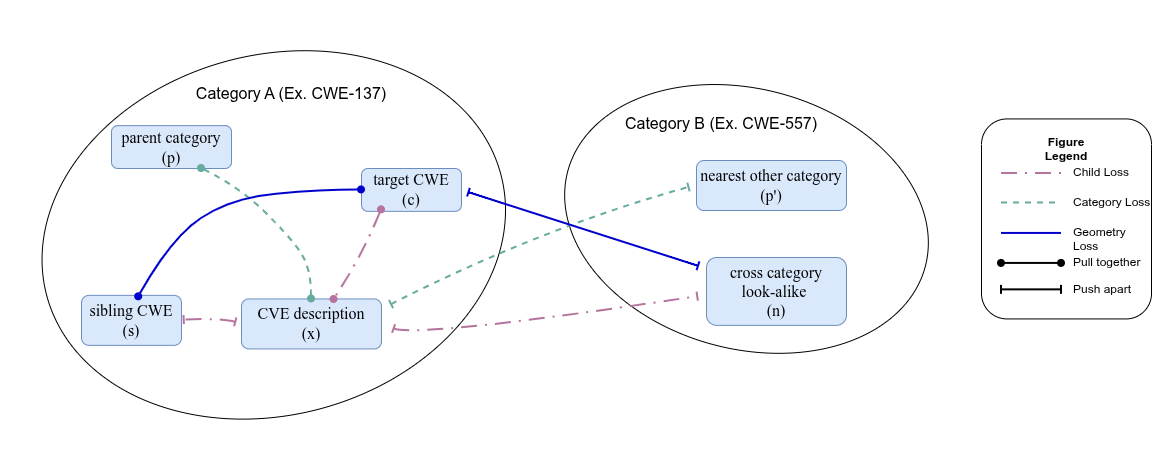
\includegraphics[width=\textwidth]{Figures/methodology/training.png}
    \caption{All three hierarchy-aware training objectives in one shared embedding space. Color and line style identify the loss; rounded-heads pull nodes together and flat bars push them apart. The three losses sum to \(\mathcal{L}\).}
    \label{fig:training_objectives}
\end{figure*}


\textbf{Training objectives.} Let \(f_\theta\) be the shared encoder, \(x\) a CVE description, \(c\) its child CWE, \(p\) a parent category, \(s\) a sibling CWE, and \(n\) a cross-category look-alike. Let \(p'\) denote the nearest other category. All CVE descriptions and CWE nodes are encoded by the same \(f_\theta\) into one shared embedding space, so every arrow in Figure~\ref{fig:training_objectives} compares vectors in that same space. Pulling two nodes together means increasing their cosine similarity; pushing them apart means decreasing it. The figure uses color and line style to distinguish the three objectives, with rounded heads for a pull and flat bars for a push.

Each objective is contrastive: it has one positive and several negatives. The negatives combine the explicit hard negatives shown in the figure with the other elements of the batch. All three objectives use the same contrastive form and differ only in their anchor, positive, and negative sets. The three objectives are:
\begin{itemize}
\item \textbf{Child} \(\mathcal{L}_{\text{child}}\): anchor \(x\), positive \(c\), negatives a sibling \(s\) and a cross-category look-alike \(n\) mined with the untuned encoder. It pulls \(x\) toward \(c\) and pushes it away from \(s\) and \(n\).
\item \textbf{Category} \(\mathcal{L}_{\text{cat}}\): anchor \(x\), positive \(p\), negative the nearest other category \(p'\). It pulls \(x\) toward \(p\) and pushes it away from \(p'\).
\item \textbf{Geometry} \(\mathcal{L}_{\text{geo}}\): anchor \(c\), positive a sibling \(s\), negative a cross-category look-alike \(n\), with no CVE involved. It pulls \(c\) toward \(s\) and pushes it away from \(n\).
\end{itemize}
The total loss is \(\mathcal{L}=\mathcal{L}_{\text{child}}+\mathcal{L}_{\text{cat}}+\mathcal{L}_{\text{geo}}\), optimized by proportional sampling over the three training sets. The child and category objectives place a CVE near both its specific weakness and its parent; the geometry objective pulls siblings together and pushes look-alikes from other categories apart. This is the sense in which HiCWE is hierarchy-aware. In an ablation under an identical budget, replacing the three objectives with plain (CVE, CWE) pairs and in-batch negatives reduces category hit@1 from 0.893 to 0.369 and end-to-end hit@1 from 0.861 to 0.324 on the internal test split (Appendix Table~\ref{tab:hierarchy_ablation}), while flat child hit@1 changes only from 0.880 to 0.831.




\textbf{Inference.} CVE and CWE nodes are encoded independently, and cosine similarity ranks the candidates; the final match is the nearest CWE rather than a generated answer. Because some children have several parents, the hierarchical child search keeps the top \(B\) categories (we use \(B=20\) of 40) and ranks the children below them; \(B=40\) recovers flat ranking. With this wide beam the hierarchical and flat child rankings are essentially identical (0.789 vs. 0.789 at \(k=1\)), so the hierarchy does its work in training rather than in the inference constraint. The flat ranking over all 399 children is therefore the primary result, and the hierarchical variant is reported for completeness. Because the CWE side is an index rather than a classification head, new definitions can be added without retraining.

\textbf{Implementation.} We fine-tune \texttt{all-MiniLM-L6-v2} and \texttt{all-MiniLM-L12-v2} with LoRA (rank 64, \(\alpha=128\), dropout 0) on the query, key, value, and dense projections, then merge the adapters so that inference is performed in a single forward pass. We train for 3 epochs with batch size 64, learning rate \(10^{-4}\), 5\% linear warmup, maximum sequence length 512, and a fixed seed; the batch sampler prevents duplicate CWE texts, and the best epoch is selected on validation end-to-end hit@3. We hold out 10\% of the 1999--2021 CVEs for validation and a separate 10\% for the internal ablation; the 2023--2025 test set is never used for tuning. Child nodes are rendered from their description and extended description; category nodes are derived from their title, summary, and immediate-child titles. CVE descriptions are normalized only during training; evaluation uses the raw NVD description.

We base our training data on the CVE--CWE mapping dataset of Liu et al.~\cite{liu2024cvecwedataset}, enriched with CWE descriptions and parent-category information from the scraped CWE-699 taxonomy (current snapshot). We train on CVEs disclosed from 1999 to 2021 and evaluate on CVEs disclosed from 2023 to 2025. This temporal split keeps the training and test  sets disjoint---no CVE appears in both sets---so it measures generalization to vulnerabilities disclosed after training, not memorization of the training set.

\textbf{Pre-processing.} Vulnerability descriptions often contain product names, vendor names, and version numbers that correlate strongly with specific CVEs, so a model can learn to ``recognize'' a vulnerability by memorizing these surface cues rather than understanding the flaw itself. Such shortcuts do not generalize to new products and would inflate our results. To force the model to learn the technical mechanism, we apply a rule-based filter to each description: we delete parenthetical text (typically patch advice), remove capitalized words that contain a lowercase letter (e.g., \texttt{Apache}, \texttt{Log4j2}) except for sentence-initial words and a whitelist of vulnerability-class terms and acronyms (e.g., SQL, HTTP, JSON, LDAP), and strip alphanumeric tokens containing a digit, which removes version numbers and names such as \texttt{log4j-core}. The filter is applied to training descriptions only; evaluation uses the raw NVD description, so the reported accuracy reflects deployment on unfiltered text. An audit found 591 of the 70,004 test descriptions (0.84\%) containing an explicit CWE identifier; because evaluation uses the raw text, these cases can inflate accuracy by at most 0.84 percentage points.

Figure~\ref{fig:cwe_dependency_graph} shows the dependency graph of the CWE-699 view, which reveals that some children belong to more than one category; the inference procedure above handles this by keeping a beam of categories rather than a single parent.


\textbf{Training set and baselines.} After filtering, the 1999--2021 training split contains 60,092 CVEs spanning 146 CWE children grouped under 35 categories (181 nodes); 25 children belong to more than one category. Table~\ref{tab:train_test_split} summarizes label coverage; the 2023--2025 test set contains 70,004 CVEs. For baselines, we use the untuned \texttt{all-MiniLM-L6-v2} and \texttt{all-MiniLM-L12-v2} encoders, which isolate the contribution of fine-tuning, and the publicly available \texttt{cwe-predictor}~\cite{mullikencwepredictor}, a DistilBERT classifier over 232 CWE labels whose flat child ranking we map to categories. We chose MiniLM because it is small, cheap to run, and available in two sizes within one family.

\begin{table}[t]
\centering
\caption{Label coverage of the CWE-699 training and test sets. All 399
children are ranked at inference, but only the 304 that occur in the
test period can be scored as labels.}
\label{tab:train_test_split}
\small
\setlength{\tabcolsep}{4pt}
\begin{tabular}{@{}l r@{}}
\toprule
\multicolumn{2}{@{}l}{\textbf{Train (1999--2021)}} \\
\midrule
CWE children with labels              & 146 \\
\midrule
\multicolumn{2}{@{}l}{\textbf{Test (2023--2025)}} \\
\midrule
CWE-699 children ranked as candidates & 399 \\
\quad appearing as test labels        & 304 \\
\qquad thereof unseen in training     & 161 \\
\addlinespace
CVEs, primary CWE seen in training    & 97.9\% \\
CVEs, primary CWE unseen              & 2.11\% \\
\bottomrule
\end{tabular}
\end{table}


Unlike keyword- or rule-based matchers, which rely on curated keyword lists and exact string overlap, HiCWE encodes the CVE description and each CWE node with the same encoder and ranks candidates by cosine similarity. This allows it to match paraphrases (e.g., ``improper neutralization'' versus ``injection'') and previously unseen phrasing without hard-coded rules. Figure~\ref{fig:methodology} summarizes the data preparation: CVE descriptions are normalized, CWE nodes are rendered as described above, and both sides are encoded by the shared bi-encoder.

\begin{figure}[!t]
    \centering
    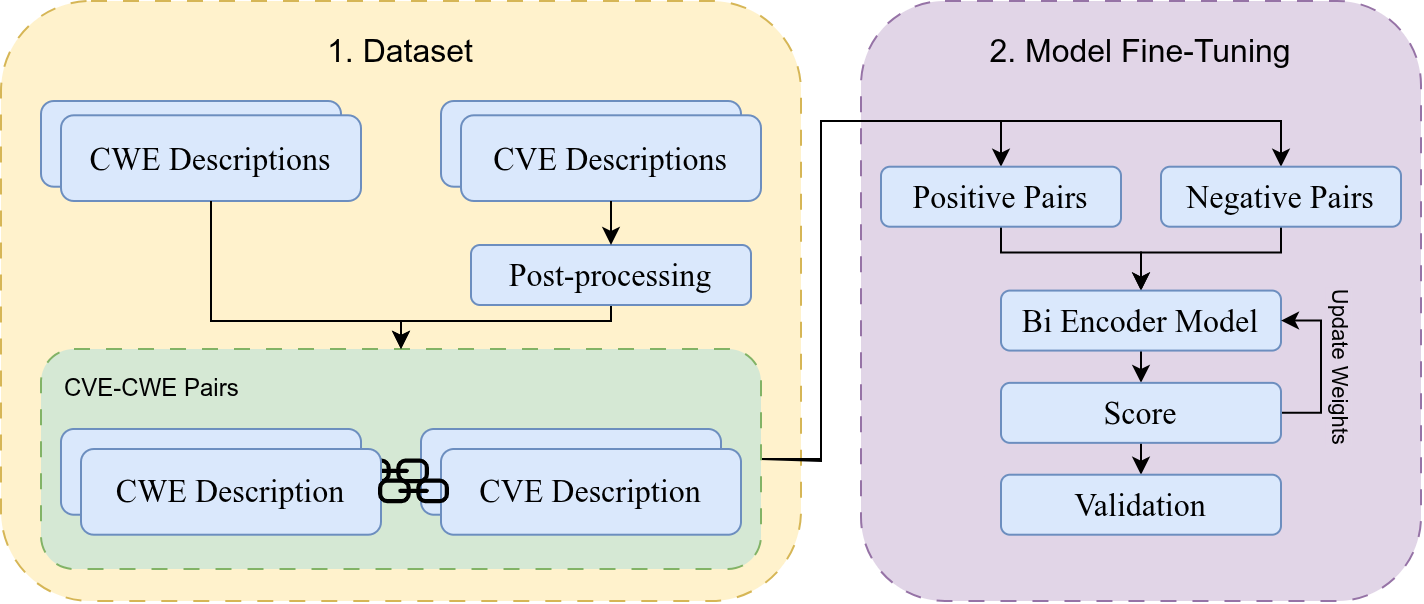
\includegraphics[width=\columnwidth]{Figures/methodology/methodology.png}
    \caption{Overview of the HiCWE pipeline: CVE descriptions and CWE nodes are encoded by a shared bi-encoder and ranked by cosine similarity.}
    \label{fig:methodology}
\end{figure}

\begin{table}[t]
\centering
\caption{CVE$\rightarrow$CWE Accuracy@$k$ on 2023--2025 CVEs (unseen during training). Best value per column in bold.}
\label{tab:accuracy}
\begin{tabular}{llccc}
\toprule
 &  & @1 & @3 & @5 \\
\midrule
\multirow[c]{6}{*}{Category} & Majority class & 0.473 & 0.668 & 0.749 \\
 & Baseline (MiniLM L6) & 0.235 & 0.408 & 0.508 \\
 & Baseline (MiniLM L12) & 0.418 & 0.634 & 0.738 \\
 & Finetuned (MiniLM L6) & 0.763 & 0.865 & 0.896 \\
 & Finetuned (MiniLM L12) & \textbf{0.820} & \textbf{0.888} & \textbf{0.913} \\
 & SOTA (cwe-predictor) & \textbf{0.820} & 0.875 & 0.881 \\
\cline{1-5}
\multirow[c]{6}{*}{Child (hier.)} & Majority class & 0.289 & 0.478 & 0.560 \\
 & Baseline (MiniLM L6) & 0.350 & 0.436 & 0.478 \\
 & Baseline (MiniLM L12) & 0.397 & 0.486 & 0.532 \\
 & Finetuned (MiniLM L6) & 0.774 & 0.840 & 0.862 \\
 & Finetuned (MiniLM L12) & \textbf{0.789} & \textbf{0.852} & \textbf{0.872} \\
 & SOTA (cwe-predictor) & 0.678 & 0.775 & 0.799 \\
\cline{1-5}
\multirow[c]{6}{*}{Child (flat)} & Majority class & 0.289 & 0.478 & 0.560 \\
 & Baseline (MiniLM L6) & 0.362 & 0.453 & 0.497 \\
 & Baseline (MiniLM L12) & 0.395 & 0.482 & 0.526 \\
 & Finetuned (MiniLM L6) & 0.771 & 0.839 & 0.862 \\
 & Finetuned (MiniLM L12) & \textbf{0.789} & \textbf{0.852} & \textbf{0.873} \\
 & SOTA (cwe-predictor) & 0.678 & 0.775 & 0.799 \\
\cline{1-5}
\bottomrule
\end{tabular}
\par\smallskip
\begin{minipage}{\columnwidth}
\footnotesize
Note: SOTA has no hierarchy stage, so its Child (hier.) row repeats its flat numbers for comparison. Category accuracy ties at 0.820 (both shown in bold). SOTA denotes the publicly available \texttt{cwe-predictor}, not a claim of state-of-the-art performance.
\end{minipage}
\end{table}

Table~\ref{tab:accuracy} reports Accuracy@$k$ at the category, hierarchy-restricted child, and flat-child levels; a hit means any ground-truth CWE is in the top-$k$. The published classifier (SOTA) is a flat 232-label classifier whose category score is derived from predicted children; it has no hierarchy-restricted child stage. \textbf{Effect of encoder size:} The untuned L12 model is stronger than the untuned L6 model, but after finetuning, the gap narrows substantially. Gains in category and child accuracy from L6 to L12 are small, and child accuracy is essentially unchanged. This suggests that the training data, rather than model capacity, is the limiting factor.

HiCWE gives the strongest child predictions; Figure~\ref{fig:accuracy} in the Appendix shows the full Accuracy@$k$ curves.

\textbf{Fine-grained capability.} Top-1 accuracy is dominated by frequent weaknesses such as cross-site scripting and SQL injection and can hide poor performance on rare CWEs. The majority-class baseline illustrates this: it reaches 0.473 category Accuracy@1 yet only 0.001 macro-F1. HiCWE's advantage is largest where classification is hardest---on rare weaknesses. HiCWE-L12 reaches a macro-F1 of 0.225 versus 0.069 for the published classifier and 0.071--0.077 for the untuned encoders (macro-F1 is computed over the 304 test labels, with predictions outside that label set counted as errors). On the tail half of the CWE distribution, HiCWE-L12 reaches 0.216 accuracy where the published classifier reaches 0.000, and it also leads on the head half (0.787 versus 0.680). Its flat MRR is 0.829 (0.814 for L6, 0.732 for the classifier, and 0.461 for the best untuned encoder).

Relative to the published systems in Section~\ref{subsec:automated_mapping}, these numbers are not directly comparable because each study fixes its own label set, split, and matching rule. The protocols closest to our evaluation are strict exact matching on temporally held-out data and the external CTI-Bench evaluation. Under that reading, HiCWE-L12 reaches 0.820 at the category level and 0.789 at the child level, against 0.678 for the published classifier at the child level; both exceed CVE2CWE's 69.9\% over a 25-way closed set and Mosievskiy's 75.6\% strict CTI-Bench top-1, while ranking all 399 children and using unfiltered NVD labels. V2W-BERT's 97\% is the only higher figure, but it combines relaxed hierarchical matching with a random partition that places same-year CVEs in both training and test; its strict equivalent is 89.2\% and its temporal result is 94\%, and its corpus overlaps our 2023--2025 test period, so we treat it as context rather than a baseline.

% \textbf{End-to-end simulation.} To test whether predicted CWEs preserve the prioritization signal, we replace the official CWE with HiCWE top-1/top-3/top-5 predictions for 2021--2025, recompute the historical exploitation score of Eq.~\ref{eq:historical_exploitability} from prior years only, and rank the CVEs of each year. We compare the official-CWE ranking, a no-CWE fallback (the global historical rate), and random ranking; the protocol and code are in \texttt{experiments/end\_to\_end\_simulation.ipynb}. The simulation is a conservative check when run with the public CISA KEV labels; the full three-source labels are used in the empirical study above.

\subsubsection{Error Analysis}

\begin{figure*}[t]
\centering
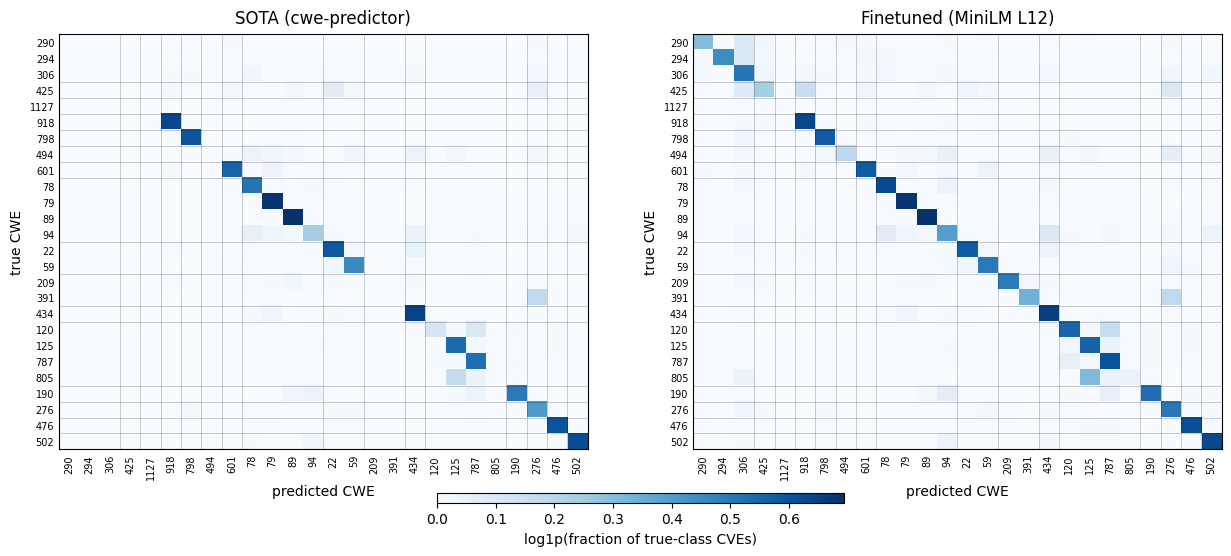
\includegraphics[width=\textwidth]{Figures/confusion_matrix.png}
\caption{Top-1 confusion matrices for the SOTA classifier (left) and HiCWE-L12 (right) over the most frequent CWEs, ordered by parent category. Rows are true CWEs and columns are predicted CWEs.}
\label{fig:confusion}
\end{figure*}


Figure~\ref{fig:confusion} shows the top-1 confusion matrices for the published classifier (left) and HiCWE-L12 (right) over the most frequent CWEs, ordered by parent category; rows are true CWEs and columns are predicted CWEs. Two patterns stand out. First, the bulk of the error sits in diagonal blocks---that is, between siblings within the same parent category, such as CWE-120/125/787 (memory-buffer weaknesses) and CWE-78/79/89 (command injection, XSS, and SQL injection)---rather than between unrelated categories. Second, the published classifier concentrates its predictions on a few frequent head classes, so for several CWEs the number of CVEs predicted to a class differs sharply from the number whose ground truth is that class; HiCWE spreads its predictions more evenly across the true labels, which is why its macro-F1 and tail accuracy exceed the classifier's. Beyond these label shifts, the published classifier has a structural coverage limit: it is trained over a fixed set of 232 CWE categories, so it cannot name any weakness outside that set---including the 253 CWE-699 children that never appear in our training corpus. HiCWE, by contrast, ranks all 399 children by similarity, so an unseen CWE can still be surfaced when its definition resembles the CVE description.


\subsection{Why Not Use Generative LLMs for CWE Mapping?}
\label{subsec:generative_llm_limitations}


LLMs, such as ChatGPT,
offer a straightforward approach to automated CVE-to-CWE
mapping: given a vulnerability description, the model
can be prompted to identify the corresponding software
weakness. Previous research has investigated the use of
prompt-based LLMs for vulnerability description mapping,
including CWE identification~\cite{liu2023not}.
However, CWE classification requires selecting a precise
identifier from a large, hierarchical taxonomy containing
semantically overlapping weaknesses. Generative models
may confuse CWE identifiers and definitions, select
overly general weakness categories, or produce
inconsistent predictions. To further investigate whether
prompt-based generative LLMs provide sufficiently reliable
CWE assignments, we conducted a preliminary experimental
evaluation of several locally deployed models.


We evaluated Llama 3.2 (3B), Qwen 2.5 (14B),
Qwen 2.5-Coder (14B), and Phi-4 (14B) using randomly selected CVEs with their NVD CWE assignments
as reference labels. Preliminary experiments showed
that allowing LLMs to generate CWE identifiers
without an explicit candidate list frequently
resulted in confusion between CWE identifiers,
names, and descriptions. We therefore developed
a constrained, hierarchy-aware prompting pipeline
that supplied official CWE identifiers, titles,
and descriptions. 

Configuration A uses a two-stage approach, selecting one
category from 40 CWE-699 categories as parent CWE and then identifying
the most relevant child CWE. Configuration B expands
the parent candidate set to 156 software-related CWEs
by incorporating 116 additional Pillar- and Class-level
weaknesses from CWE-699. Configuration C reduces error
propagation by selecting the top three parent candidates,
combining their children, and performing a final selection
over the resulting candidate set.



The initial evaluation on 25 CVEs revealed limited
classification accuracy for both models. Under
Configuration A, Llama 3.2 (3B) achieved 0\%
exact-match accuracy, while Qwen 2.5 (14B) achieved
4\%. Expanding the taxonomy in Configuration B
improved exact-match accuracy to 12\% and 16\%,
respectively. However, Llama 3.2 repeatedly predicted
the same CWE for 24 of the 25 CVEs, indicating that
its apparent improvement did not reflect reliable
weakness discrimination. Moreover, both configurations
restricted classification to the children of a single
predicted parent, making an incorrect initial selection
difficult to recover from.

To address this limitation, Configuration C retains
the three most relevant parent candidates and performs
a final selection among their combined children.
In the initial evaluation, Qwen 2.5 achieved 20\%
exact-match accuracy under Configuration C, compared
with 16\% under Configuration B. Although Llama 3.2's
accuracy decreased to 8\%, its prediction diversity
improved substantially. Based on these findings,
we selected Configuration C for further evaluation
on a larger dataset of 1000 CVEs to assess its
performance across additional LLM architectures.


Table~\ref{tab:generative_llm_summary} summarizes exact-match and parent-level accuracy for Configuration C over 1,000 CVEs. At $T=0$, Qwen 2.5-Coder
achieved the highest exact-match accuracy (23.3\%)
and parent-level accuracy (28.0\%), outperforming
Qwen 2.5 (17.3\% and 20.7\%), Phi-4 (16.7\%
and 16.0\%), and Llama 3.2 (7.3\% and 9.3\%).
Adjusting the decoding temperature improved
Qwen 2.5-Coder's exact-match accuracy to 26.0\%
at $T=0.3$. Furthermore, enriching the CVE
description with information retrieved from
external reference links increased exact-match
accuracy to 32.0\% and parent-level accuracy
to 32.7\%, although average processing time
increased from 3.9 to 6.4 seconds per CVE.
The results of the temperature sensitivity experiments
under Configuration C for the four evaluated LLMs are
reported in Tables~\ref{tab:temperature_all}, in the Appendix.

Despite these refinements, the best-performing
generative configuration correctly identified
the exact CWE for only 32.0\% of the evaluated
vulnerabilities. Moreover, 10.7\% of the
reference CWE assignments were outside the
evaluated taxonomy, illustrating the importance
of candidate coverage. These findings suggest
that prompt engineering, hierarchical reasoning,
and contextual enrichment alone do not guarantee
reliable fine-grained CWE identification.
The observed sensitivity to model selection,
taxonomy construction, and decoding parameters
also complicates the use of generative models
as a consistent automated classification mechanism.

These limitations motivate our investigation of
a lightweight, fine-tuned bi-encoder as an
alternative to generative CWE prediction.
Rather than generating CWE identifiers through
autoregressive decoding, the proposed approach
learns semantic representations of CVE descriptions
and CWE definitions and ranks predefined candidate
weaknesses according to their similarity.
This design avoids unconstrained identifier
generation and provides a deterministic
candidate-ranking mechanism.


\begin{table}[t]
\centering
\caption{Generative LLM performance for CVE-to-CWE
mapping ($n=1000$). Results use Configuration C
and $T=0$, unless otherwise specified.}
\label{tab:generative_llm_summary}
\scriptsize
\setlength{\tabcolsep}{3pt}
\begin{tabular}{lrr}
\toprule
\textbf{Model}
& \textbf{Exact (\%)}
& \textbf{Parent (\%)} \\
\midrule
Llama 3.2 (3B)        & 7.3  & 9.3 \\
Qwen 2.5 (14B)        & 17.3 & 20.7 \\
Phi-4 (14B)          & 16.7 & 16.0 \\
Qwen 2.5-Coder (14B)  & 23.3 & 28.0 \\
\midrule
Qwen 2.5-Coder ($T=0.3$)
                       & 26.0 & 26.7 \\
+ Reference enrichment ($T=0.3$)
                       & 32.0 & 32.7 \\
\bottomrule
\end{tabular}
\par\smallskip
\begin{minipage}{\columnwidth}
\footnotesize
Note: exact-match is computed over all evaluated CVEs; parent-level accuracy is computed over the subset whose reference CWE has a parent in the evaluated taxonomy, so the two denominators differ.
\end{minipage}
\end{table}


Note that the evaluated generative
LLMs may have encountered some of the CVE descriptions
and their corresponding CWE assignments during
pretraining, as this information is publicly available
through vulnerability databases. Although the extent
of such exposure cannot be verified, the possibility
of training-data overlap makes the relatively low
classification accuracy particularly noteworthy.
Even with potential prior exposure to some CVE--CWE
mappings, the best-performing configuration achieved
only 32.0\% exact-match accuracy. This observation
further motivates the development of a task-specific
CWE classification approach.

To address this concern in our proposed bi-encoder
evaluation, we adopt a temporal data-splitting
strategy, using CVEs published between 1999 and
2021 for training and CVEs published between 2023
and 2025 for testing. This separation prevents
direct overlap between the CVE records used for
fine-tuning and those used for evaluation, providing
a more realistic assessment of the model's ability
to generalize to newly disclosed vulnerabilities.

To facilitate reproducibility, all prompts used in
the generative LLM experiments, together with the
implementation and evaluation scripts, are publicly
available in our repository.


% \section{Exploitability Ranking Using Historical CWE Exploitability Score}
% \label{sec:exploitability-ranking}

% To evaluate the practical usefulness of historical weakness-level exploitability, we conducted a temporal exploitability ranking experiment. Unlike supervised exploitability prediction models, the objective of this experiment is to determine whether historical exploitation patterns associated with software weaknesses (CWEs) can provide a useful signal for prioritizing newly disclosed vulnerabilities. This experiment also establishes a foundation for evaluating our LLM-based framework, in which official CWE assignments can subsequently be replaced with automatically predicted CWE labels.

% We used the official CVE--CWE mappings provided by the National Vulnerability Database (NVD). A vulnerability was considered exploited if it appeared in at least one of the exploitation datasets used in this study: CISA Known Exploited Vulnerabilities (KEV), VulnCheck, or GreyNoise.

% For each evaluation year, historical exploitability scores were estimated using vulnerabilities published before that year. Specifically, for each CWE $c$, the historical exploitation probability was calculated as

% \begin{equation}
% P(\mathrm{Exploited}\mid c)=
% \frac{E_c+\alpha P_0}{N_c+\alpha},
% \label{eq:historical_exploitability}
% \end{equation}

% where $E_c$ denotes the number of historically exploited CVEs mapped to CWE $c$, $N_c$ represents the total number of historical CVEs associated with that CWE, $P_0$ is the overall historical exploitation rate, and $\alpha$ is a smoothing parameter.

% The smoothing parameter reduces the influence of sparse observations, preventing CWEs with only a few historical CVEs from receiving unreliable exploitation estimates. We evaluated $\alpha \in \{20,40,60\}$ and observed improvements when increasing $\alpha$ from 20 to 40, with negligible additional changes at 60. Therefore, we selected $\alpha=40$ for the remaining experiments.

% Each CVE $v$ was assigned the historical exploitation score of its associated CWE. When multiple CWE assignments existed, the maximum score was used:

% \begin{equation}
% \mathrm{RankScore}(v)=
% \max_{c \in \mathrm{CWE}(v)}
% P(\mathrm{Exploited}\mid c),
% \label{eq:ranking_score}
% \end{equation}

% where $\mathrm{CWE}(v)$ denotes the set of CWE assignments associated with vulnerability $v$. CVEs were ranked in descending order of their historical exploitability scores. CVEs without usable CWE assignments received the global historical exploitation rate as a fallback score.

% We adopted a rolling temporal evaluation strategy covering 2021--2025. For each test year, historical CWE exploitation probabilities were calculated from CVEs published in preceding years, while evaluation was performed exclusively on CVEs published during the corresponding year. For example, the 2023 evaluation used historical CWE exploitation estimates derived from CVEs published before 2023.

% Ranking performance was evaluated using the Area Under the Precision--Recall Curve (PR-AUC), Area Under the ROC Curve (ROC-AUC), Precision@$k$, Recall@$k$, and Normalized Discounted Cumulative Gain (NDCG@$k$), with $k \in \{50,100,250,500\}$. PR-AUC was considered the primary metric because exploited vulnerabilities represent a small fraction of disclosed CVEs. The different cutoffs reflect varying vulnerability remediation capacities.

% Since multiple CVEs can share identical CWE-based exploitability scores, deterministic ranking may introduce arbitrary ordering among tied vulnerabilities. To address this limitation, we performed 1,000 random tie-breaking iterations, randomly permuting CVEs with identical scores while preserving the ordering of distinct score levels. We report the expected Precision@$k$, Recall@$k$, and NDCG@$k$ averaged across these iterations.

% \textbf{Results--}
% Table~\ref{tab:cwe_ranking} summarizes the temporal
% exploitability ranking performance using official NVD
% CWE assignments and compares it against random ranking.
% The CWE-based approach achieved ROC-AUC values ranging
% from 0.6919 to 0.7268 and PR-AUC values ranging from
% 0.0352 to 0.0520 across the five evaluation years.
% Although the absolute PR-AUC values were relatively low,
% they consistently exceeded the random ranking baselines
% of 0.0127 to 0.0226, corresponding to improvements
% of approximately 2.20 to 2.77 times.

% Similarly, CWE-based Precision@100 ranged from 0.0571
% to 0.0990, outperforming the random ranking baselines
% by factors of approximately 3.14 to 7.78.
% These results suggest that historical CWE exploitation
% patterns provide useful information for vulnerability
% prioritization despite the low prevalence of exploited
% vulnerabilities.

% \begin{table*}[t]
% \centering
% \caption{Temporal exploitability ranking using official NVD CWE
% assignments compared with random ranking. CWE P@100, R@100,
% and NDCG@100 are averaged over 1,000 random tie-breaking
% iterations. Random ranking baselines are based on the
% yearly prevalence of exploited CVEs.}
% \label{tab:cwe_ranking}
% \scriptsize
% \begin{tabular}{lrrrrrrrrrr}
% \toprule
% \textbf{Year} &
% \textbf{CVEs} &
% \textbf{Exploited} &
% \textbf{ROC-AUC} &
% \multicolumn{2}{c}{\textbf{PR-AUC}} &
% \multicolumn{2}{c}{\textbf{P@100}} &
% \textbf{R@100} &
% \textbf{NDCG@100} &
% \textbf{Coverage} \\
% \cmidrule(lr){5-6}
% \cmidrule(lr){7-8}
% & & & & \textbf{CWE} & \textbf{Random}
% & \textbf{CWE} & \textbf{Random} & & & \\
% \midrule
% 2021 & 21,019 & 476 & 0.6919 & 0.0520 & 0.0226 & 0.0852 & 0.0226 & 0.0179 & 0.0859 & 79.9\% \\
% 2022 & 25,793 & 448 & 0.7016 & 0.0466 & 0.0174 & 0.0961 & 0.0174 & 0.0214 & 0.0967 & 84.5\% \\
% 2023 & 29,377 & 534 & 0.7036 & 0.0401 & 0.0182 & 0.0571 & 0.0182 & 0.0107 & 0.0571 & 88.4\% \\
% 2024 & 40,484 & 677 & 0.7161 & 0.0408 & 0.0167 & 0.0696 & 0.0167 & 0.0103 & 0.0693 & 93.2\% \\
% 2025 & 49,549 & 631 & 0.7268 & 0.0352 & 0.0127 & 0.0990 & 0.0127 & 0.0157 & 0.0986 & 90.1\% \\
% \bottomrule
% \end{tabular}
% \end{table*}

% Table~\ref{tab:cwe_precision_cutoffs} in Appendix, presents expected Precision@$k$ across four prioritization cutoffs. Precision remained relatively stable across cutoffs of 50, 100, 250, and 500 during 2021--2024, suggesting that groups of vulnerabilities with identical or similar CWE-based scores occupy substantial portions of the highest-ranked positions. In 2025, Precision decreased from 0.0994 at $k=50$ to 0.0721 at $k=500$, indicating greater concentration of exploited vulnerabilities among the highest-ranked CVEs.

% Overall, these findings demonstrate that historical CWE exploitation frequencies provide a meaningful prioritization signal, while also revealing a limitation of weakness-level scoring: vulnerabilities sharing the same CWE may receive identical scores despite having different exploitation outcomes. Consequently, the approach is more suitable for identifying higher-risk weakness categories than for finely distinguishing individual vulnerabilities.

% \textbf{Comparison with EPSS--}
% To further assess the usefulness of historical CWE-based
% exploitability scores for vulnerability prioritization,
% we compared their predictive performance with EPSS using
% PR-AUC and Precision@100 on matched CVEs and exploitation
% labels. As shown in Table~\ref{tab:cwe_epss_comparison},
% EPSS consistently outperformed the CWE-based approach,
% achieving a mean PR-AUC of 0.3755 compared with 0.0436
% and a mean Precision@100 of 0.7880 compared with 0.0815.
% This difference was expected, as EPSS incorporates multiple
% vulnerability-specific signals, whereas our approach relies
% solely on historical weakness-level exploitation patterns.
% Nevertheless, the CWE-based approach demonstrated predictive
% value beyond random ranking, supporting its potential as
% an interpretable and complementary signal for vulnerability
% prioritization.


% \begin{table}[t]
% \centering
% \caption{Comparison of historical CWE-based exploitability scores and EPSS on matched CVEs (2021--2025).}
% \label{tab:cwe_epss_comparison}
% \small
% \begin{tabular}{lcccc}
% \toprule
% \textbf{Year} &
% \multicolumn{2}{c}{\textbf{PR-AUC}} &
% \multicolumn{2}{c}{\textbf{P@100}} \\
% \cmidrule(lr){2-3}
% \cmidrule(lr){4-5}
% & \textbf{CWE} & \textbf{EPSS} &
% \textbf{CWE} & \textbf{EPSS} \\
% \midrule
% 2021 & 0.0533 & 0.4193 & 0.0851 & 0.78 \\
% 2022 & 0.0472 & 0.3298 & 0.0963 & 0.64 \\
% 2023 & 0.0408 & 0.3974 & 0.0579 & 0.77 \\
% 2024 & 0.0410 & 0.3313 & 0.0688 & 0.84 \\
% 2025 & 0.0355 & 0.3995 & 0.0996 & 0.91 \\
% \midrule
% \textbf{Mean} &
% \textbf{0.0436} & \textbf{0.3755} &
% \textbf{0.0815} & \textbf{0.7880} \\
% \bottomrule
% \end{tabular}
% \end{table}


% Notably, EPSS scores were obtained from an October 2026 snapshot; therefore, the comparison is retrospective rather than temporally aligned. The CWE-based results in Table~\ref{tab:cwe_ranking}
% are calculated using the complete yearly CVE datasets,
% whereas Table~\ref{tab:cwe_epss_comparison} reports
% results on the subset of CVEs with available EPSS scores
% and nonzero historical CWE-based scores. Consequently,
% minor differences in CWE ranking performance arise from
% the different evaluation populations and random
% tie-breaking procedures. These results should therefore not be interpreted as directly equivalent evaluations.

% Nevertheless, historical CWE exploitation frequencies demonstrated predictive value relative to random ranking. The objective of this experiment is therefore not to replace EPSS, but to assess whether weakness-level exploitation history can provide an interpretable and potentially complementary signal for vulnerability prioritization.


\section{Limitations and Threats to Validity}

Like all empirical studies, this work has several limitations. Our analysis assumes that CWE assignments in the NVD accurately represent the underlying software weaknesses. Although Finding 2 showed that few CWE mappings change after publication, some may still be incomplete, overly coarse, or incorrect. The mapping guidance itself changed over time: CVEs from 1999--2021 are disproportionately assigned to coarse weaknesses such as CWE-119, CWE-20, and CWE-264, whereas 2023--2025 CVEs use more specific base-level weaknesses. The 2023--2025 test set mitigates this temporal label shift but does not eliminate it. Similarly, exploitability was identified using CISA KEV, VulnCheck, and GreyNoise. While combining these sources improves coverage, exploited vulnerabilities absent from all three datasets may be incorrectly classified as non-exploited, and recently disclosed CVEs may not yet be classified as exploited even though they could be in the future.

The CWE taxonomy is a snapshot of the current CWE-699 Software Development view, which contains 40 categories and 399 children. CVEs whose assigned CWE is absent from this view are dropped from training and evaluation, so deprecated or out-of-view weaknesses do not enter the analysis; this keeps the label space consistent but removes weaknesses that were historically common. Coverage is also uneven: only 146 of the 399 children appear as labels in the 1999--2021 corpus, and the other 253 are ranked at inference but never seen as positives. We regard this as a strength of the retrieval formulation rather than a limitation: because HiCWE ranks all 399 children by similarity instead of selecting from a fixed label set, it can still surface an unseen CWE when its definition resembles the CVE description, whereas a fixed-label classifier cannot name such a weakness at all. The practical impact is small---in the 2023--2025 test set, only 1,478 CVEs (2.11\%) have an unseen primary CWE (1,544, or 2.21\%, by any label), while 97.9\% have a primary CWE seen during training. About 11\% of CVEs carry more than one CWE; counting a hit on any ground-truth CWE measures recall but can overstate exact label agreement, and a stricter all-label metric would be lower.

Methodological choices may also influence the results. Historical exploitability analyses considered only CWE-year combinations with sufficient observations, and exploitability rankings were restricted to CWEs satisfying minimum sample-size and statistical significance requirements. Although sensitivity analyses showed that the identified CWEs remain largely consistent under different thresholds, alternative thresholds or ranking weights may produce different rankings. Likewise, the LLM evaluation used specific prompting strategies, taxonomy configurations, and a limited set of open-source models; different prompts, models, or retrieval methods may yield different results, and the framework targets software weaknesses defined by the CWE taxonomy, so it may require adaptation for other vulnerability taxonomies. In addition, we fine-tuned only the MiniLM L6 and L12 embedding models and did not evaluate other base encoders because of compute constraints, so the findings may not generalize to larger or architecturally different embedding models. We also report a single training run per encoder size and do not estimate variance across seeds, which limits claims about the stability of the reported gains.

For the CWE-mapping evaluation, the post-processing filter is applied to training descriptions only; evaluation uses the raw NVD description, so the reported numbers reflect deployment on unfiltered text rather than the normalized training distribution. The filter removes explicit CWE identifiers such as CWE-79 from training text but not from evaluation text, so an explicit identifier in a test description would be a potential leak; we audit the test set for such cases. On the comparison side, the published classifier is trained on the same source corpus, but its label space and preprocessing differ from ours, so it is not a perfectly controlled baseline. We report V2W-BERT, CVE2CWE, the RoBERTa-based classifier, and the fine-tuned models of Simonetto et al. as published context rather than as baselines: their label spaces, splits, and matching rules differ from ours, and their training corpora overlap our 2023--2025 test period or are not publicly available. Finally, Accuracy@1 is dominated by frequent weaknesses; we therefore report macro-F1, per-CWE results, and a head-versus-tail split, which are less sensitive to the head of the distribution.

Our empirical study relies on publicly disclosed CVEs from the NVD and publicly available exploitation datasets. Consequently, undisclosed vulnerabilities or exploits known only through proprietary threat intelligence are not represented, limiting generalizability to private vulnerability repositories or organization-specific environments. Finally, although we observed statistically significant temporal stability of historical exploitability at the CWE level, the correlations are moderate rather than strong. Historical exploitability should therefore be viewed as one informative signal rather than a complete predictor of exploitation. It is intended to complement other factors, including CVSS metrics, affected products, exploit availability, and threat intelligence, in future vulnerability prioritization frameworks. Moreover, the evaluation measures CWE classification accuracy rather than the end-to-end performance of a vulnerability prioritization system; an evaluation of early vulnerability prioritization is future work.

\section{Conclusion and Future Work}
\label{sec:conclusion}

We investigated the use of historical CWE exploitability patterns and automated CWE classification for early vulnerability prioritization. Our empirical analysis of 192,788 CVEs revealed significant differences in exploitation rates across CWE categories and moderate temporal stability (mean Spearman's $\rho=0.480$), showing the potential of historical weakness-level information as a prioritization signal. We introduced HiCWE, a hierarchy-aware contrastive bi-encoder for automated CVE-to-CWE mapping, achieving 82.0\% top-1 category accuracy and 78.9\% fine-grained accuracy, outperforming the evaluated baselines and a published classifier at the fine-grained level. HiCWE fine-tunes the MiniLM L6 and L12 embedding models and ranks CWE descriptions directly by cosine similarity; because it has no fixed classification head, new or revised weaknesses can be added by updating the CWE index rather than retraining the model. We also showed that historical CWE exploitation rates provide a consistent ranking signal for future vulnerabilities, achieving ROC-AUC scores between 0.692 and 0.727 across temporal evaluations from 2021 to 2025 using official NVD CWE assignments.

Future work will focus on evaluating the complete framework by incorporating HiCWE-predicted CWE labels into the exploitability ranking process. We also plan to investigate multi-label CWE classification, improve generalization to rare and newly introduced weaknesses, evaluate larger embedding backbones, and integrate historical CWE exploitability with complementary indicators such as CVSS, EPSS, and threat intelligence to improve prioritization accuracy.

Our findings show that historical CWE exploitability provides a useful complementary signal for early vulnerability prioritization and that hierarchy-aware semantic learning can improve automated weakness identification.



\clearpage
\bibliographystyle{IEEEtran}
\bibliography{references.bib}

\clearpage
\section*{Appendix}

\begin{table}[!htbp]
\centering
\caption{Training-objective ablation with the L6 base model on the internal 1999--2021 test split (random 10\% hold-out). These numbers are not comparable to Table~\ref{tab:accuracy}, which uses the temporal 2023--2025 test set.}
\label{tab:hierarchy_ablation}
\small
\begin{tabular}{lrrr}
\toprule
\textbf{Metric} & \textbf{Baseline} & \textbf{Child-only} & \textbf{Full} \\
\midrule
Category hit@1 & 0.152 & 0.369 & 0.893 \\
Category hit@3 & 0.294 & 0.629 & 0.952 \\
Child oracle hit@1 & 0.444 & 0.891 & 0.937 \\
End-to-end hit@1 & 0.033 & 0.324 & 0.861 \\
Flat child hit@1 & 0.189 & 0.831 & 0.880 \\
Flat MRR & 0.289 & 0.873 & 0.913 \\
\bottomrule
\end{tabular}
\end{table}

\begin{figure}[!htbp]
\centering
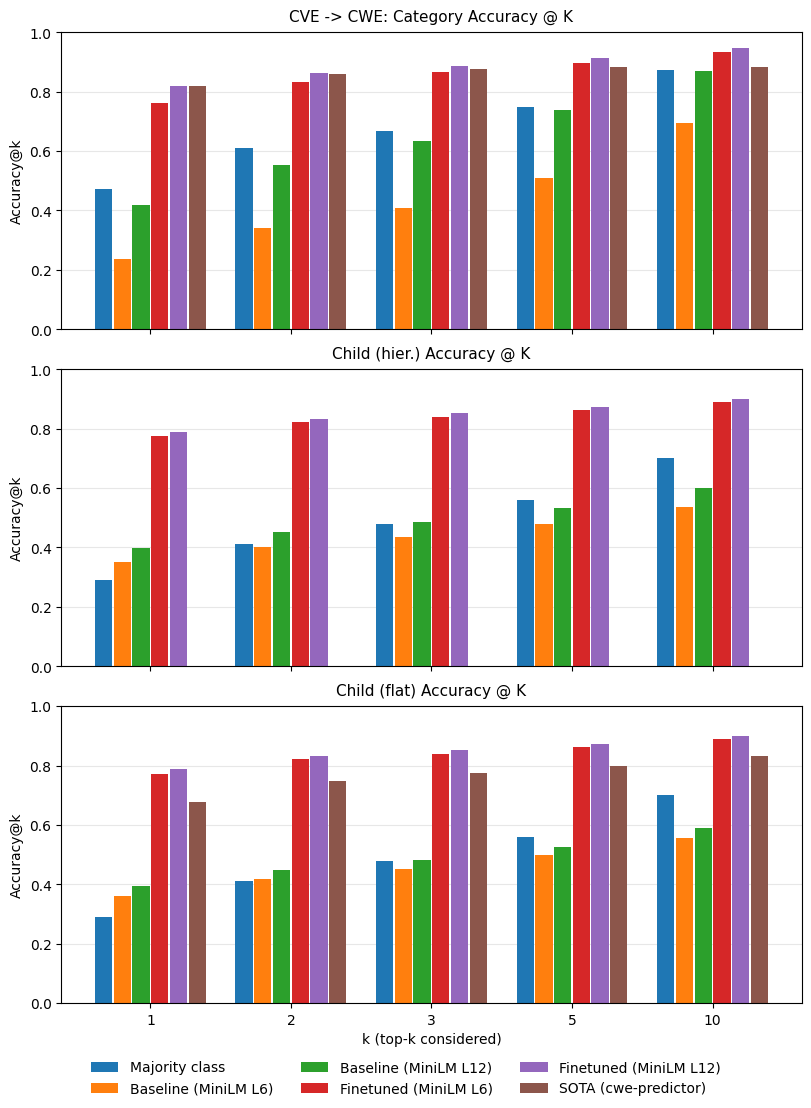
\includegraphics[width=\columnwidth]{Figures/model/overall.png}
\caption{CVE$\rightarrow$CWE Accuracy@$k$ for the untuned baseline, the fine-tuned models, and the published classifier; one panel per target.}
\label{fig:accuracy}
\end{figure}

\begin{table}[!htbp]
\centering
\caption{Top 25 CWEs by Mapped Known Exploited Vulnerabilities 2025}
\label{tab:kev_top25}
\begin{tabular*}{\columnwidth}{@{\extracolsep{\fill}}lr@{}}
\toprule
\textbf{CWE ID} & \textbf{Mapped KEVs} \\
\midrule
78 & 18 \\ 502 & 15 \\ 22 & 13 \\ 416 & 11 \\ 787 & 11 \\
77 & 7 \\ 79 & 7 \\ 287 & 6 \\ 288 & 6 \\ 306 & 6 \\
94 & 6 \\ 122 & 5 \\ 125 & 5 \\ 121 & 4 \\ 20 & 4 \\
284 & 4 \\ 36 & 4 \\ 434 & 4 \\ 843 & 4 \\ 862 & 4 \\
863 & 4 \\ 89 & 4 \\ 119 & 3 \\ 120 & 3 \\ 506 & 3 \\
\bottomrule
\end{tabular*}
\end{table}

\begin{table}[!htbp]
\centering
\caption{Expected Precision@$k$ under random tie-breaking across different prioritization cutoffs.}
\label{tab:cwe_precision_cutoffs}
\small
\begin{tabular*}{\columnwidth}{@{\extracolsep{\fill}}lcccc@{}}
\toprule
\textbf{Year} & \textbf{P@50} & \textbf{P@100} & \textbf{P@250} & \textbf{P@500} \\
\midrule
2021 & 0.0853 & 0.0852 & 0.0853 & 0.0859 \\
2022 & 0.0982 & 0.0961 & 0.0962 & 0.0963 \\
2023 & 0.0564 & 0.0571 & 0.0568 & 0.0572 \\
2024 & 0.0700 & 0.0696 & 0.0688 & 0.0687 \\
2025 & 0.0994 & 0.0990 & 0.0765 & 0.0721 \\
\bottomrule
\end{tabular*}
\end{table}


\begin{figure}[!htbp]
    \centering
    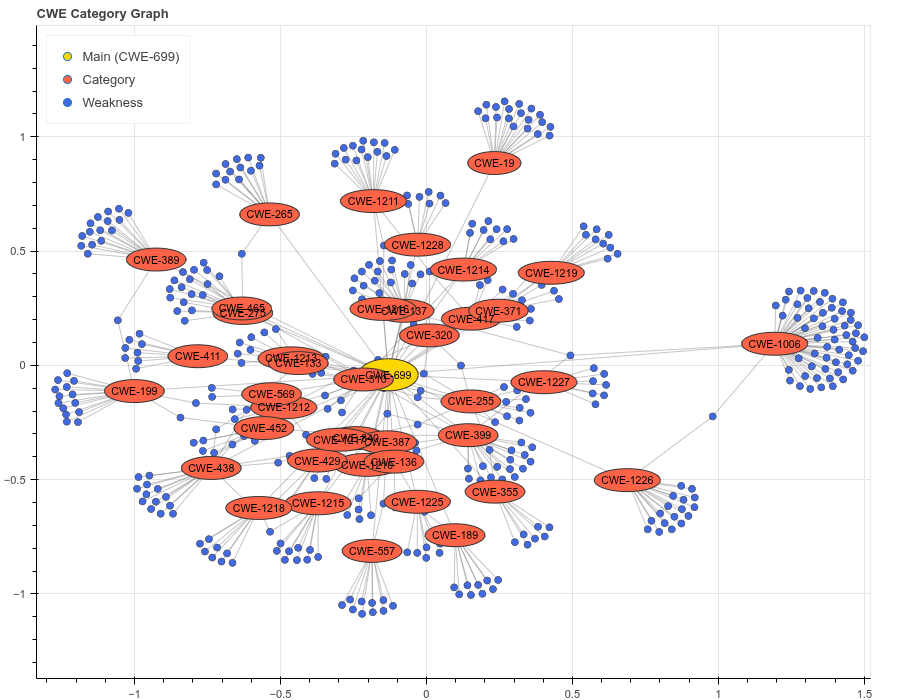
\includegraphics[width=\columnwidth]{Figures/methodology/cwe_dependency_graph.png}
    \caption{Dependency graph of the CWE-699 Software Development view. Edges link categories to their children; children with multiple parents appear under more than one category, which motivates keeping a beam of categories rather than a single parent.}
    \label{fig:cwe_dependency_graph}
\end{figure}

\onecolumn

\begin{table}[!htbp]
\centering
\caption{Temperature sensitivity of the evaluated LLMs under Configuration C.}
\label{tab:temperature_all}
\small
\begin{tabular*}{\columnwidth}{@{\extracolsep{\fill}}llcccc@{}}
\toprule
\textbf{Model} & \textbf{Metric} &
\textbf{T=0.0} & \textbf{T=0.3} & \textbf{T=0.7} & \textbf{T=1.0} \\
\midrule
\multirow{3}{*}{qwen2.5-coder (14B)}
& Exact-match accuracy  & 23.3\% & 26.0\% & 25.3\% & 19.3\% \\
& Parent-level accuracy & 28.0\% & 26.7\% & 30.7\% & 22.7\% \\
& Avg.\ time (s/CVE)    & 3.9 & 3.9 & 3.8 & 3.8 \\
\midrule
\multirow{3}{*}{qwen2.5 (14B)}
& Exact-match accuracy  & 17.3\% & 14.0\% & 18.0\% & 16.7\% \\
& Parent-level accuracy & 20.7\% & 16.7\% & 21.3\% & 20.0\% \\
& Avg.\ time (s/CVE)    & 3.8 & 3.7 & 3.6 & 3.6 \\
\midrule
\multirow{3}{*}{phi4 (14B)}
& Exact-match accuracy  & 16.7\% & 16.7\% & 16.7\% & 16.7\% \\
& Parent-level accuracy & 16.0\% & 18.0\% & 18.0\% & 16.7\% \\
& Avg.\ time (s/CVE)    & 5.6 & 5.3 & 5.3 & 5.4 \\
\midrule
\multirow{3}{*}{llama3.2 (3B)}
& Exact-match accuracy  & 7.3\% & 5.3\% & 3.3\% & 2.0\% \\
& Parent-level accuracy & 9.3\% & 6.7\% & 4.7\% & 2.0\% \\
& Avg.\ time (s/CVE)    & 1.2 & 1.2 & 1.2 & 1.1 \\
\bottomrule
\end{tabular*}
\end{table}

\end{document}
